% Options for packages loaded elsewhere
\PassOptionsToPackage{unicode}{hyperref}
\PassOptionsToPackage{hyphens}{url}
\PassOptionsToPackage{dvipsnames,svgnames,x11names}{xcolor}
%
\documentclass[
  12pt,
]{book}
\usepackage{amsmath,amssymb}
\usepackage{iftex}
\ifPDFTeX
  \usepackage[T1]{fontenc}
  \usepackage[utf8]{inputenc}
  \usepackage{textcomp} % provide euro and other symbols
\else % if luatex or xetex
  \usepackage{unicode-math} % this also loads fontspec
  \defaultfontfeatures{Scale=MatchLowercase}
  \defaultfontfeatures[\rmfamily]{Ligatures=TeX,Scale=1}
\fi
\usepackage{lmodern}
\ifPDFTeX\else
  % xetex/luatex font selection
\fi
% Use upquote if available, for straight quotes in verbatim environments
\IfFileExists{upquote.sty}{\usepackage{upquote}}{}
\IfFileExists{microtype.sty}{% use microtype if available
  \usepackage[]{microtype}
  \UseMicrotypeSet[protrusion]{basicmath} % disable protrusion for tt fonts
}{}
\makeatletter
\@ifundefined{KOMAClassName}{% if non-KOMA class
  \IfFileExists{parskip.sty}{%
    \usepackage{parskip}
  }{% else
    \setlength{\parindent}{0pt}
    \setlength{\parskip}{6pt plus 2pt minus 1pt}}
}{% if KOMA class
  \KOMAoptions{parskip=half}}
\makeatother
\usepackage{xcolor}
\usepackage[margin=3cm]{geometry}
\usepackage{longtable,booktabs,array}
\usepackage{calc} % for calculating minipage widths
% Correct order of tables after \paragraph or \subparagraph
\usepackage{etoolbox}
\makeatletter
\patchcmd\longtable{\par}{\if@noskipsec\mbox{}\fi\par}{}{}
\makeatother
% Allow footnotes in longtable head/foot
\IfFileExists{footnotehyper.sty}{\usepackage{footnotehyper}}{\usepackage{footnote}}
\makesavenoteenv{longtable}
\usepackage{graphicx}
\makeatletter
\def\maxwidth{\ifdim\Gin@nat@width>\linewidth\linewidth\else\Gin@nat@width\fi}
\def\maxheight{\ifdim\Gin@nat@height>\textheight\textheight\else\Gin@nat@height\fi}
\makeatother
% Scale images if necessary, so that they will not overflow the page
% margins by default, and it is still possible to overwrite the defaults
% using explicit options in \includegraphics[width, height, ...]{}
\setkeys{Gin}{width=\maxwidth,height=\maxheight,keepaspectratio}
% Set default figure placement to htbp
\makeatletter
\def\fps@figure{htbp}
\makeatother
\setlength{\emergencystretch}{3em} % prevent overfull lines
\providecommand{\tightlist}{%
  \setlength{\itemsep}{0pt}\setlength{\parskip}{0pt}}
\setcounter{secnumdepth}{5}
\usepackage{booktabs}
\ifLuaTeX
  \usepackage{selnolig}  % disable illegal ligatures
\fi
\usepackage[]{natbib}
\bibliographystyle{apalike}
\IfFileExists{bookmark.sty}{\usepackage{bookmark}}{\usepackage{hyperref}}
\IfFileExists{xurl.sty}{\usepackage{xurl}}{} % add URL line breaks if available
\urlstyle{same}
\hypersetup{
  pdftitle={CHAPTER 9: ANALYSIS OF HOUSEHOLD SURVEY DATA},
  pdfauthor={Andrés Gutiérrez, Pedro Luis do Nascimento Silva},
  colorlinks=true,
  linkcolor={blue},
  filecolor={Maroon},
  citecolor={Blue},
  urlcolor={Blue},
  pdfcreator={LaTeX via pandoc}}

\title{CHAPTER 9: ANALYSIS OF HOUSEHOLD SURVEY DATA}
\author{Andrés Gutiérrez\footnote{Comisión Económica para América Latina y el Caribe (CEPAL) - \href{mailto:andres.gutierrez@cepal.org}{\nolinkurl{andres.gutierrez@cepal.org}}}, Pedro Luis do Nascimento Silva\footnote{SCIENCE, \href{mailto:pedronsilva@gmail.com}{\nolinkurl{pedronsilva@gmail.com}}}}
\date{2025-01-07}

\begin{document}
\maketitle

{
\hypersetup{linkcolor=}
\setcounter{tocdepth}{0}
\tableofcontents
}
\listoffigures
\listoftables
\hypertarget{abstract}{%
\chapter*{Abstract}\label{abstract}}
\addcontentsline{toc}{chapter}{Abstract}

Analyzing complex household survey data requires knowing and properly applying the foundations of \emph{design-based inference}. The researcher will be faced to a small dataset containing information that will allow her to make conclusions over the whole population.

The purpose of any analysis on this kind is not to make conclusions about the sample itself -- which in most of the cases is a small subset of the population - but to the the whole population and possibly domains or population subgroups of interest. Having that into account, the first step in any analysis plan should be devoted to understanding and specifying the sampling design used to draw the sample and the findings on the field related to nonresponse and lack of coverage.

This chapter covers three main topics of analysis: descriptive statistics; comparisons and associations; and modeling of survey data. First, we introduce simple descriptive statistics, such as totals, means, frequencies and proportions, quantiles and some graphics; next, we delve deeper on relationships between the survey variables. All these analyses rely on the representativity principle of the design-based inference. This way, the reader will find a strong focus, not only on point estimates, but also on uncertainty measures. The chapter also presents a short discussion on the different approaches that can be used to estimate variances; the best way to visualize the estimates; and some NSO practical experiences.

\hypertarget{introduction}{%
\chapter*{Introduction}\label{introduction}}
\addcontentsline{toc}{chapter}{Introduction}

A key concern for every agency that produces statistical information is ensuring the \emph{correct} use of the data it provides. This concern is enshrined in the United Nations \emph{Fundamental Principles of Official Statistics}, particularly in the following principles:

\begin{itemize}
\tightlist
\item
  \textbf{Principle 3:} To facilitate a correct interpretation of the data, statistical agencies must present information according to scientific standards, including details on the sources, methods, and procedures used.
\item
  \textbf{Principle 4:} Statistical agencies are entitled to comment on erroneous interpretation and misuse of statistics.
\end{itemize}

The advent of the computer revolution, coupled with greater access to computational tools, has led to increased use of statistical data, including household survey data. Sometimes this data is used for mostly \emph{descriptive purposes}, such as estimating population means or obtaining estimates of population frequency distributions. Other times, however, its use is made for \emph{analytical purposes}, involving the testing of hypothesis or the construction of models, when the objective is to draw conclusions that are also applicable to populations other than the one from which the sample was extracted. When using standard statistical software for such analyses, results can be biased or misleading if the complex sampling design is not properly accounted for.

Household surveys also play a critical role in tracking progress toward global objectives, such as the \textbf{Sustainable Development Goals (SDGs)}. For this purpose, descriptive analyses often include a range of specialized indicators designed to monitor outcomes like access to education, health services, and economic opportunities. These indicators are derived from the survey data and are essential for policymakers and organizations aiming to achieve sustainable development targets.

This chapter aims to empower users to analyze household survey data accurately and effectively. It does this by presenting relevant models, methods, and software that enables the data analyst to understand key steps in the data analysis process and to incorporate complex designs into their analyses. It relies on the fundamental concepts of the design-based paradigm for survey design and analysis.

What makes household survey data special or challenging for those who intend to analyse them is because they are collected through complex sampling methods that often involve:

\begin{itemize}
\tightlist
\item
  \textbf{Stratification}: Dividing the population into comprehensive distinct subgroups before sampling;
\item
  \textbf{Clustering}: Grouping units and sampling groups rather than units to simplify data collection;
\item
  \textbf{Unequal probabilities of selection}: Giving units different probabilities of being selected;
\item
  \textbf{Weighting adjustments}: Correcting for non-response and/or improving precision.
\end{itemize}

Standard data analysis methods and software ignore these features, leading to biased estimates of both the target parameters and their associated variances. Here we analyze the impact of simplifications made when using standard data analysis methods and software, and present the necessary adjustments to these methods in order to appropriately incorporate the aspects highlighted above into the analysis.

Different readers of the chapter may find some of its parts more useful than others. Here we describe contents of each of the sections, so that readers may direct their attention to the topics of relevance to them. Section 9.1 provides guidance on the preparation of a plan for the analysis of the household survey data. Such plans are important both to guide survey development and subsequently any secondary survey data analysis.

Section 9.2 provides a short discussion on the fundamental principles of the design-based inference, emphasizing that conclusions taken from probability sample surveys should be based on a pair: the point estimate and it associated margin of error (or any related measure). Section 9.3 begins the journey with the key tools for descriptive analysis: means, ratios, proportions and other typical descriptive parameters.

Section 9.4 is devoted to more complex parameters that allow comparisons of the phenomenon of interest between subgroups for continuous and discrete variables. It also presents standard tests to compare means and measure the degree of correlation and association between variables.

Section 9.5 focuses on modelling survey outcomes. It starts with a discussion on the role of weighting when estimating regression coefficients, followed by presentation of some proper approaches to estimate complex parameters in linear and logistic regression models. Finally, section 9.6 presents a summary of ideas and tools for survey data visualization, showing the best practices for creating graphics in a context where sampling imbalance and uncertainty are important.

Throughout the chapter, practical examples are provided to illustrate how National Statistics Offices (NSOs) conduct various types of household survey data analysis. These examples provide a useful guide for applying the concepts and methods discussed in real-world contexts. By the end of the chapter, readers will be equipped with the knowledge and tools needed to analyze household survey data effectively while accounting for the complexities of survey designs adopted in such surveys.

\hypertarget{planning-and-preparation-for-analysis}{%
\chapter{Planning and Preparation for Analysis}\label{planning-and-preparation-for-analysis}}

Planning the analysis stage of a survey is an essential part of the overall survey planning process. Following the \textbf{Generic Statistical Business Process Model (GSBPM)} (\url{https://unece.org/statistics/documents/2019/01/standards/gsbpm-v51}), this step corresponds to the subprocess labeled as \emph{2.1 - Design Outputs}.

At this stage, it is important to distinguish between two groups of users: primary data producers and secondary data users. Proper planning and understanding of the survey design are crucial for both. For primary data producers, creating a comprehensive tabular plan ensures alignment with survey objectives. For secondary users, clear research questions and attention to survey metadata enable accurate and meaningful analyses.

\hypertarget{primary-data-producers}{%
\section{Primary data producers}\label{primary-data-producers}}

They are responsible for planning and executing the survey to collect the intended data. For them, planning the analysis typically involves preparing a \emph{tabular plan} --- a document specifying the core set of tables to be produced once the survey data becomes available. This plan helps to ensure that the survey results align with the stated needs and objectives of the survey (see chapter 2). It also helps those designing the survey questionnaire(s) to ensure that all items needed are included, and possibly, help avoid adding items / questions that are not really needed for the intended analysis (see chapter 4).

Preparing a \emph{tabular plan} generally requires defining three sets of specifications:

\begin{enumerate}
\def\labelenumi{\arabic{enumi}.}
\item
  \textbf{Filter Conditions}: These may be used to define subgroups of the population for which specific tables will be produced. For example, in a survey where questions regarding occupation are asked only from individuals aged 15 or older, a filter condition might be `if age \textgreater{} 14'. Such a condition means that only those in the relevant age group would be included in tables for the occupation related variables (status, type, income, etc.).
\item
  \textbf{Classification or Domain Variables}: These are variables used to subdivide the population into meaningful groups for analysis. For example, geographic areas (e.g., states or provinces), age groups, or sex might define rows in a table. These variables are often chosen to meet reporting requirements, such as providing estimates by province in national household surveys. A typical list of domain defining variables would include: geographic levels (provinces, etc.); type of region (urban x rural); sex; age groups; education; race / etchnicity; etc.
\item
  \textbf{Response or Survey Variables}: These are the variables being analyzed to understand how they vary across the defined domains. For instance, continuous survey variables (like income) might be used to create columns in a table, summarizing means, medians, or other statistics. These variables are all others that we do not use as classification ones. Categorical survey variables (like employment status) will generate a column for each category where the corresponding cross-classified frequencies will appear, with one row for each of the classes of the domain defining variables.
\end{enumerate}

As discussed throughout Chapter 7, an important consideration when defining domains is related to sample design, particularly when defining strata and sample sizes. For most national household sample surveys, providing breakdowns by province or state is required, and therefore stratification by province will be essential. Additionally, if precision requirements must be met at the provincial level, sample sizes that satisfy these requirements must be computed for each province and then summed to obtain the national sample size.

For instance, for domains defined by characteristics that are unavailable from the sampling frame, say age groups, for the case of household surveys that use area sampling, sample size calculations must take into account what the required total sample size must be such that estimates for the rarest group meet precision specifications. As an example, suppose that estimates are required by age groups such as young adults (18 to 29), adults (30 to 49), ageing adults (50 to 59) and elderly (60 and over). Assuming that the population distribution by these age groups is such that the ageing adults is the rarest group with 12.5\% of the total population, and if a minimum sample size of 500 individuals in this group is required, then the total sample must be at least 500 / 0.125 = 4,000. That is, in order for the full sample to provide an expected sample of about 500 ageing adults we must sample at least 4,000 individuals for the survey.

\hypertarget{secondary-data-users}{%
\section{Secondary Data Users}\label{secondary-data-users}}

Secondary data users are all those who will access and analyze the survey data after it has been released, typically with access only to the public datasets and documentation provided by the data producers or curators. Their first task is to define clear research questions and locate the relevant survey data and documentation (metadata). Good survey metadata must describe the sampling design and estimation methods used (including details about stratification, clustering, and survey weights), both for descriptive parameters and for the corresponding measures of precision.

For example, based on the aforementioned, a well-defined research question posed by some secondary data user, can be such as \textbf{``Do rural households face digital exclusion compared to urban households?''}. Notice that it directs the analysis towards estimating relevant parameters and precision measures.

The question might involve testing whether the proportion of rural households with internet access is significantly lower than that of urban households. This clarity allows for more direct and accurate analyses. The null hypothesis behind this question is that \(H_0) P_{Rural} = P_{Urban}\), which we wish to test against the alternative \(H_A) P_{Rural} < P_{Urban}\), where \(P\) denotes the proportion of households having internet access in the domain identified.

A related but different set of hypothesis could be \(H_0) C_{Rural} = C_{Urban}\) versus \(H_A) C_{Rural} > C_{Urban}\) where \(C\) denotes the average cost of connection for broadband internet access in the specified domain. Listing the research questions in this way would enable the subsequent analysis to progress more directly towards the estimation of the relevant parameters from the survey data, and corresponding precision measures, both of which are required to compute test statistics that would provide the evidence required to answer them.

In order for such estimation to take place, the secondary data user must first find out details about how the sampling was conducted so that the user can incorporate the sampling design features provided in the database during the analysis stage. As we will discuss in subsequent sections of this chapter, it is essential to account for the survey weights (see Chapter 8) when computing point estimates of both descriptive and model parameters, and to account for the structural components of the sampling design and estimation process (stratification, clustering, unequal inclusion probabilities, non-response adjustment, and calibration of survey weights, if any) when estimating variances or other measures of precision for the point estimates.

Users that disregard such aspects of the sampling design do so at their peril, and may end up producing biased estimates that will lead to incorrect inferences and decisions. The recommended practice is for data producers to provide sufficient detail about such sampling aspects as part of the metadata released with survey microdata, in order to enable secondary data users to consider these aspects when conducting their analyses of interest.

\hypertarget{quality-control-for-secondary-users}{%
\section{Quality Control for Secondary Users}\label{quality-control-for-secondary-users}}

A standard quality control process for secondary data users would consist of the following steps:

\begin{enumerate}
\def\labelenumi{\arabic{enumi}.}
\item
  \textbf{Load the Data and Metadata}: Ensure that the survey microdata is properly linked to metadata describing the key aspects of the sampling design (stratification and clustering identifiers, unequal probabilities of selection) and estimation processes (weights, replicate weights if any, non-response correction, calibration, etc.).
\item
  \textbf{Replicate Published Estimates}: Recreate some of the estimates provided by the survey producers, including measures of precision, to confirm that the data and sampling design aspects have been correctly interpreted and loaded.
\item
  \textbf{Compare Scenarios}: When the user is capable of replicating published estimates, she can then proceed towards the required new analysis for which no previous results are available. Repeat this analysis under two scenarios: ignoring and accounting for the sampling design. Compare the results and assess the impact of incorporating the sample design.
\item
  \textbf{Finalize the Analysis}: Use only the results that account for the sampling design in the final interpretation, ensuring that the design effects are appropriately incorporated.
\end{enumerate}

\hypertarget{accounting-for-the-sampling-design}{%
\chapter{Accounting for the Sampling Design}\label{accounting-for-the-sampling-design}}

When analysing household survey data, ignoring the sampling design undermines the representativeness, accuracy, and credibility of survey-based findings, which can lead to incorrect decisions. This is why accounting for the sampling design is essential when analyzing household survey data to ensure valid and unbiased estimates. As seen in the previous chapters, regular household surveys have two major characteristics:

\begin{itemize}
\item
  They use \emph{complex sampling designs} (e.g., stratification, clustering, and unequal probabilities of selection) to represent the population efficiently.
\item
  They define \emph{sampling weights} for each sampling unit (primary, and remaining ones) to properly represent the population.
\end{itemize}

To illustrate this fact, we provide a simple example. Suppose a country has two regions: Region A with 100 people, and Region B with 900 people. Wealthy people live in Region A, with an average income of \$10,000, less wealthy people live in Region B, with average income of \$2,000. The true population average income is \$2,800, because:

\[
\theta = \frac{(100 \times 10,000) + (900 \times 2,000)}{100 + 900} = 2,800.
\]

Suppose a survey is conducted where 50 people are sampled from each Region. After data collection, it was found that the sample mean for Region A was \$10,000, while the sample mean for Region B was \$2,000. If the sampling design is ignored, all units in the sample will receive equal weights, regardless of their corresponding population sizes. This way, the average income is estimated with severe bias as:

\[
\hat \theta = \frac{(50 \times 10,000) + (50 \times 2,000)}{100} = 6,000.
\]

despite the fact that both sample averages within regions are perfect estimates of the corresponding population averages.

When the sampling design is considered, weights are applied proportional to the population sizes of each region. This way, units in Region A would receive a weight of \(\frac{100}{50} = 2\), while units in Region B would receive a weight of \(\frac{900}{50} = 18\). In this escnario, the average income is unbiasedly estimated as:

\[
\hat \theta = \frac{(2 \times 50 \times 10,000) + (18 \times 50 \times 2,000)}{(2 \times 50) + (18 \times 50)} = 2,800.
\]

Ignoring the sampling design (and corresponding weights) causes that Region A (smaller but wealthier) dominates the estimate, even though its population represents only 10\% of the country's population. This creates a bias, making the average population income seem higher than it actually is. By considering the sampling design (the sample was stratified by region, with equal allocation), and using weights, the latest estimate correctly reflects the true contribution of each Region to the global average, thus avoiding bias.

Another crucial aspect to take into account is clustering. Most household sample surveys select an area sample, with clusters defined by census enumeration areas or similar groups of households. Then from within each sampled cluster, a sub-sample of households is selected for the survey. While such designs are cost efficient, they imply some loss in precision for the resulting estimates.

Consider a toy example where clusters are city blocks, and a sample of 10 households is selected within each cluster to be surveyed. Suppose the target parameter is the proportion of households which have electricity provided from a city grid. Assuming that each cluster either is included or excluded from the grid, a sample of 1,000 households obtained from such a design would be as precise as sample of only 100 households, if they were sampled by simple random sampling. The reason is that after observing a single household in each cluster, the other 9 we sample there are not brining in any new information. Any analysis of the full sample of households would fool the user to believe that the estimates are as precise as having sampled 1,000 households at random from the population, which was not the case, and standard errors would be severely underestimated.

In real applications, to enable adequate analysis that accounts for the sampling design, survey datasets must contain identifiers for strata and primary sampling units (PSU), as well as weights for relevants units of analysis (households, individuals, etc.). Alternatively, when such information is not available, the dataset should at least contain replicate weights, and the user should have clear guidance on how to compute both point and variance estimates.

This section discusses how survey data from a sample can be used to draw conclusions about an entire population using a design-based approach. This approach assumes that the sample is selected through a well-defined probability sampling process, which ensures that every unit in the population has a known, non-zero chance of being sampled. Sampling weights, which reflect how much each sampled unit represents in the population, are essential tools in this approach. These weights allow users to make estimates that account for the sampling process and produce results that are representative of the population. A well-described survey design facilitates statistical analysis, supports effective data interpretation, and enables meaningful insights into complex phenomena. Not accounting for it may lead to biased estimates and misleading conclusions, as illustrated.

\hypertarget{parameters-and-estimators}{%
\section{Parameters and Estimators}\label{parameters-and-estimators}}

Two common goals when analyzing survey data are to estimate the value of a characteristic for the whole population, such as total income, and to estimate the average value of that characteristic, such as the average income per person. These are referred to as the \emph{population total} and the \emph{population mean}, respectively. The design-based approach incorporates the probability sampling design in the inferential process.

Under probability sampling, every unit in the population has a known chance of being included in the sample. The \emph{sample inclusion probabilities} are then used to calculate \emph{basic sampling weights}. When the design is properly incorporated, estimates for population totals and means are unbiased. This means that, on average, the estimates will equal the true population values if the survey were to be repeated many times under the same conditions.

The estimators used to make inferences about the population parameters use the sampling weights to create weighted sums of the survey data, which serve as estimates for the population parameters. If the weights are appropriately applied, the resulting estimates are consistent with the true values in the population.

As stated in Chapter 8, in some situations, the basic sampling weights need adjustments to improve the accuracy of survey estimates. Adjustments may account for survey non-response, where weights of responding units are corrected to account for units that were selected for the survey but did not participate. These adjusted weights help to minimize biases in the estimates and make the results more reliable. If calibration was performed, the weights are modified to ensure that the weighted sums align more closely with known population distributions, such as age or sex distributions.

The \emph{population total} \(Y = \sum _{U} y_k\) and \emph{mean} \(\overline Y = \frac Y N\) of a survey variable \(y\) can be estimated by weighted estimators given by \(\widehat Y _{HT} = \sum _{s} d_k \ y_k\) and \(\overline y_{H} = \frac {\widehat Y_{HT}} {\widehat N_{HT}} = \frac {\sum_{s} d_k \ y_k} {\sum_{s} d_k}\), respectively. The basic design weights \(d_k = 1 / \pi_k\) are given by the reciprocals of the sample inclusion probabilities of the sampled units (denoted \(\pi_k\)), for all \(k \in s\).

When the survey weights are calibrated and/or non-response adjusted, the above expressions may still be used, but with the calibrated or non-response adjusted weights, \(w_k\) say, replacing the basic design weights \(d_k\), for all \(k \in s\).

Here \(s = \left\{ k_1, \ldots, k_n \right\} \subset U\) denotes the set of units in a sample selected from the population \(U\) using a \emph{probability sampling design} \(p(s)\), that ensures strictly positive first order inclusion probabilities \(\pi_k = Pr(k \in s), \, \forall \, k \in U\). These inclusion probabilities are assumed known \(\forall \, k \in s\), at least to the data producers.

An important part of survey analysis is understanding the level of uncertainty in the estimates. Since we are working with a sample and not the entire population, there will always be some variability in the estimates. This variability is measured using either the \emph{sampling variance}, the \emph{standard error} or the \emph{coefficient of variation} (\emph{cv}) of the estimates. The latter two are functions of the first, and serve to indicate by how much the estimate might differ from the true population value in absolute (\emph{se}) or relative (\emph{cv}) terms. Under the design-based framework and assuming full response, \(\widehat Y _{HT}\) is unbiased for \(Y\) and its sampling variance can be estimated unbiasedly by

\[
\widehat {V_p} \left( \widehat{Y}_{HT} \right) = \sum_{k \in s} \sum_{j \in s} \left( d_k d_j - d_{kj} \right) y_k y_j
\]

Where \(d_{kj} = 1 / \pi_{kj}\) and \(\pi_{kj} = Pr(k,j \in s), \, \forall \, k,j \in U\). This result assumes that the sampling design \(p(s)\) is such that \(\pi_{kj} > 0 \,\, \forall \, k,j \in U\). Considering the sampling design is crucial for the computation of variance. For example, consider a population of size \(N = 6\), and a sample of size \(n = 3\). Let's assume that the following sample values were observed: \((y_1 = 10, y_2 = 14, y_3 = 18)\). If the sampling design is simple random sampling without replacement, the above formula becomes:

\[
\widehat {V}_{SRS} \left( \widehat{Y}_{HT} \right) = \frac{N^2}{n} \left( 1 - \frac{n}{N} \right) S^2_{y_s}
\]

Where \(S^2_{y_s}\) is the sample variance. After a simple algebraic manipulation, the formula becomes \(\widehat {V_p} \left( \widehat{Y}_{HT} \right) = \frac{36}{3} \cdot \left(1 - \frac{3}{6} \right) 16 = 96\). A naive analyst might incorrectly compute the variance using the following formula, which ignores the sampling design: \(\frac{N^2}{n}S^2_{y_s} = 192\).

Notice that the estimate for the population total is \(\widehat{Y}_{HT} = 84\). The proper standard error is \(\sqrt{\widehat {V_p} \left( \widehat{Y}_{HT} \right)} = \sqrt{96} \approx 9.80\). The 95\% confidence interval is \(84 \pm 19.25 = [64.75, 103.25]\). Using the naive variance, an incorrect 95\% confidence interval is \([56.80, 111.20]\). The naive confidence interval is wider than the correct confidence interval, and it overestimates the uncertainty in the total. This example clearly demonstrates the importance of considering the sampling design when calculating variances and confidence intervals. Ignoring the sampling design can lead to incorrect inferences.

While the formula for variance estimation \(\widehat {V_p}\) is general and covers the vast majority of sample designs used in the practice of household sample surveys, it is not used in practice because the second order inclusion probabilities \(\pi_{kj}\) (and corresponding pairwise weights \(d_{kj}\)) are generally unknown to secondary survey data users. In fact, even data producers do not compute such pairwise weights, since there are more efficient methods for variance estimation that do not require having such weights.

For this reason, simpler and more efficient methods are often used in practice, allowing users to quantify the uncertainty without requiring overly detailed information about the sampling design.

\hypertarget{approaches-to-variance-estimation}{%
\section{Approaches to Variance Estimation}\label{approaches-to-variance-estimation}}

When working with household surveys, the sample is usually only a small subset of the entire population. Because of this, it is important to provide not only the main estimates of interest, such as totals or averages, but also the level of uncertainty in these estimates.

Understanding and estimating uncertainty is a critical part of analyzing household survey data; by using proper methods, users can measure the reliability of their estimates. There are several methods to estimate the uncertainty in survey results.

\begin{itemize}
\item
  \emph{Estimating Equations} \citep{Binder1983}, which comprises a unifying idea of sampling theory, provides a flexible framework for estimating totals, means, ratios, and other parameters as well as their corresponding variances.
\item
  \emph{Taylor Linearization} is an approach that relies on approximating complex non-linear statistics by linear ones, and then estimating the variance / se / cv of the linear approximating quantity.
\item
  The \emph{Ultimate Cluster} method is often used in surveys that collect data through stratified multi-stage sampling, and relies on computing the variance between quantities calculated at the level of the primary sampling units (PSU). It is often combined with \emph{Taylor Linearization} for obtaining estimates of variances of non-linear statistics, such as means, ratios, etc.
\item
  The \emph{Bootstrap} and other replication methods rely on sampling repeatedly from the observed sample, computing estimates from each replica, and then using the variability between the estimates to estimate the variance / se / cv of the main estimate.
\end{itemize}

With the help of modern software, all of these approaches can be implemented efficiently, ensuring accurate and meaningful analysis of survey data.

\hypertarget{estimating-equations}{%
\subsection{Estimating Equations}\label{estimating-equations}}

Many population parameters can be written/obtained as solutions of \emph{population estimating equations}. Variance estimation for these sample-based methods follows a consistent framework. Although the details can be technical, the key idea is that the same principles used to estimate totals can be applied to estimate variances. This generality makes the method simple and versatile, allowing it to be well implemented in widely used software like the \texttt{R\ survey} package and the \texttt{Stata\ svy} functions. These tools automate much of the process, making it accessible for users to estimate both population parameters and their associated uncertainties.

A generic population \emph{estimating equation} is given by \(\sum_{i \in U} z_i (\theta) = 0\), where \(z_i(\cdot)\) is an \emph{estimating function} evaluated for unit \(i\) and \(\theta\) is a population parameter of interest. These equations provide a general way to define and calculate many population parameters, such as totals, means, and ratios. The concept is straightforward: population parameters can be defined as solutions to specific equations that involve all the units in the population. This approach is flexible and can be adapted to calculate many different types of parameters.

\begin{itemize}
\item
  For the case of the population total, take \(z_i(\theta) = y_i - \theta / N\). The corresponding population estimation equation is given by \(\sum _{i \in U} (y_i - \theta / N) = 0\). Solving for \(\theta\) gives the population total \(\theta_U = \sum _{i \in U} y_i \ = \ Y\).
\item
  For ratios of population totals, taking \(z_i(\theta) = y_i - \theta x_i\), the corresponding population estimating equation is given by \(\sum _{i \in U} (y_i - \theta x_i) = 0\). Solving for \(\theta\) gives the \emph{population ratio} \(\theta_U = \sum _{i \in U} y_i / \sum _{i \in U} x_i \ = \ R\).
\item
  Similarly, for population means, take \(z_i(\theta) = y_i - \theta\).
\end{itemize}

The idea of defining population parameters as solutions to population estimating equations allows defining a general method for obtaining corresponding sample estimators. It is a matter of using the \emph{sample estimating equations} \(\sum _{k \in s} d_k \, z_k (\theta) = 0\). Under \emph{probability sampling}, full response and with \(d_k = 1 / \pi_k\), the sample sum in the left hand side is unbiased towards the population sum in the corresponding population estimating equation. Solving the sample estimating equation yields consistent estimators for the corresponding population parameters.

A consistent estimator for the variance of non-linear estimators obtained as solutions of sample estimating equations, derived using \emph{Taylor Linearization}, is given by:

\[
\widehat V_{TL} (\widehat \theta) = \left[ \widehat J ( \widehat \theta) \right] ^{-1} \widehat V_p \left[ \sum _{k \in s} d_k \, z_k (\widehat \theta)\right] \left[ \widehat J ( \widehat \theta) \right] ^{-1}
\]

Where \(\widehat J (\widehat \theta) = \sum _{k \in s} d_k \, \left[ \partial{z_k ( \theta)} / \partial \theta \right]_{\theta = \widehat \theta}\).

This approach implies that one is able to estimate many population parameters and corresponding variances using essentially well known methods for estimating totals and their variances. Its simplicity and generality have enabled the development of software such as the \texttt{R\ survey} package, the \texttt{Stata\ svy} functions and others.

\hypertarget{ultimate-cluster}{%
\subsection{Ultimate Cluster}\label{ultimate-cluster}}

The \emph{Ultimate Cluster} is a straightforward and powerful approach for estimating the variance of totals in surveys that use stratified multi-stage cluster sampling designs. This method, proposed by \citet{Hansen1953}, simplifies the complex nature of multi-stage designs by focusing only on the variation between the largest groups, known as Primary Sampling Units (PSUs). It assumes that, within each sampling stratum, PSUs were sampled independently with replacement (potentially with unequal probabilities), even if they were actually selected without replacement in the actual sampling process.

The method considers only the variation between statistics computed at the level of PSUs. This method allows for a simpler variance estimation, while still providing reliable variance estimates. This idea is simple, but quite powerful, because it allows to accommodate a variety of sampling designs, involving stratification and selection with unequal probabilities (with or without replacement) of both PSUs as well as lower level sampling units (households and individuals). The requirements for the application of this method are the following:

\begin{itemize}
\item
  Unbiased estimates of totals for the variable(s) of interest are available for each sampled PSU;
\item
  Data are available for at least two sampled PSUs in each stratum (if the sample is stratified in the first stage);
\item
  The survey dataset contains all the information regarding PSUs, strata and weights.
\end{itemize}

Consider a multi-stage sampling design, in which \(m_{h}\) PSUs are selected in stratum \(h\), with \(h=1, \ldots ,H\). Let \(\widehat{Y}_{hi} = \sum_{i \in s_{1h}} \sum_{k \in s_{hi}} d_{hik} \ y_{hik}\) denote an estimate of the population total \(Y_h\) in stratum \(h\) based on the single PSU \(i\) sampled in this stratum. Then an unbiased estimator of the population total \(Y = \sum_{h=1}^{H} \sum_{i \in U_{1h}} Y_{hi}\) is given by \(\widehat{Y}_{UC} = \sum_{h=1}^{H} \widehat{Y}_{h}\) where \(\widehat{Y}_{h} = \frac{1}{m_{h}} \sum_{i \in s_{1h}} \widehat{Y}_{hi}\). The \emph{Ultimate Cluster} estimator of the corresponding variance is given by:

\[
\widehat{V}_{UC} \left( \widehat{Y}\right) = \sum_{h=1}^{H} \frac{m_{h}}
{m_{h}-1} \sum_{i \in s_{1h}} \left( \widehat{Y}_{hi} - \widehat{Y}_{h} \right) ^{2}
\]

where \(U_{1h}\) and \(s_{1h}\) are the population and sample sets of PSUs in stratum \(h\), for \(h=1,\ldots ,H\). (See for example, \citep{Shah1993}, p.~4).

Although the method was originally proposed for estimation of variances of estimated totals, it can also be applied in combination with \emph{Taylor Linearization} and \emph{Estimating Equations} approaches to obtain variance estimates for estimators of many other population quantities that can be obtained as solutions to sample estimating equations. This makes the method versatile and useful for a wide range of applications in survey analysis.

One key assumption of the method is that, within strata, the PSUs were selected independently and with replacement. In reality, most surveys select PSUs without replacement, which provides for more efficient designs. However, the variance estimates produced by the \emph{Ultimate Cluster} method are generally close enough to be useful, even under these conditions, provided the sampling fraction of PSUs is small.

The \emph{Ultimate Cluster} method is particularly attractive because of its simplicity. Survey practitioners often prefer it over more complex approaches that account for all stages of the sampling design. Although these detailed methods may provide slightly more accurate variance estimates, they are harder to implement and require more detailed information about the sampling process. In contrast, this method offers a reasonable approximation that works well for most practical purposes, especially for estimating totals or averages. A discussion about Quality of this approximation and alternatives can be found in \citep{SSW92}, p.~153.

\hypertarget{bootstrap}{%
\subsection{Bootstrap}\label{bootstrap}}

Replication methods for variance estimation are based on the idea of re-sampling from the available sample, computing the estimates from each replica, and then using the variability between the estimates across replicas to estimate the variance. They are particularly useful when the user does not have access to information on stratum and/or PSUs identifiers in the database, and the \emph{Ultimate Cluster} method cannot be used in such cases.

The \emph{bootstrap} method comprises a powerful and flexible approach for estimating variances in surveys and many other contexts. Originally proposed by \citet{Efron1979}, the version commonly used for household surveys is called the Rao-Wu-Yue Rescaling Bootstrap \citep{Rao1992}. This method is well-suited for stratified multi-stage sampling designs and has become widely used for variance estimation with complex survey data.

Conceptually, the \emph{bootstrap} method relies on creating many new ``replicated'' datasets, which are slightly different versions of the original sample. These replicated datasets mimic the process of repeatedly drawing samples from the population. By analyzing the variation in results across these datasets, we can estimate how much uncertainty there is in our estimates from the original sample. In practice, the method can be applied by creating multiple columns of weights in the original sample data set, with weights modified to mimic the process of re-sampling from the available sample. The creation of these multiple columns of weights should be done by the National Statistical Office following the steps outlined below.

\begin{enumerate}
\def\labelenumi{\arabic{enumi}.}
\item
  First, create a new sample for each stratum by randomly selecting primary sampling units (PSUs) from the original sample, allowing PSUs to be selected more than once (with replacement). Each selected PSU is included in the new dataset along with all its associated data and lower level units. The size of this random sample with replacement is of \(m_h - 1\) PSUs in each of the \(H\) design strata.
\item
  This process of creating new samples is repeated many times, usually hundreds or thousands, to produce multiple ``replicated'' datasets. That is, repeat Step 1 \(R\) times, and denote by \(m_{hi}(r)\) the number of times that the PSU \(i\) of stratum \(h\) was selected for the sample in replicate \(r\).
\item
  For each replicate \(r\), \emph{bootstrap} weights are calculated for each unit. These weights account for how often each PSU appears in the replicate and ensure that the replicated datasets remain representative for the population. The \emph{bootstrap} weight for unit \(k\) within PSU \(i\) of stratum \(h\) in replica \(r\) is \(w_{hik}(r) = w_{hik} \times \frac {m_h}{m_h - 1} \times m_{hi}(r)\).
\item
  The parameter of interest, such as a total or mean, is estimated for each replica using the \emph{bootstrap} weights for that replica. That is, for each replica \(r\), calculate an estimate \(\widehat \theta_{(r)}\) of the target parameter \(theta\) using the \emph{bootstrap} weights \(w_{hik}(r)\) instead of the original weights \(w_{hik}\).
\item
  Finally, the variability of the results across all replicas is used to estimate the variance. The idea is that the variation in these replicate estimates reflects the uncertainty in the original estimate. This estimate of the variance takes the following form:
\end{enumerate}

\[
\widehat V_{B} \left( \widehat \theta \right) = \frac {1} {R} \sum_{r=1}^R \left( \widehat \theta_{(r)} - \tilde \theta \right)^2
\]

where \(\tilde \theta = \frac 1 R \sum_{r=1}^R \widehat \theta_{(r)}\) is the average of the replica estimates.

Whenever the original sampling weights \(w_{hik}\) receive non-response adjustments or are calibrated, the corresponding non-response adjustments and/or calibration of the basic weights must be repeated for each replica, so that the variance estimates adequately reflect the effects of the calibration and non-response adjustments on the uncertainty of the point estimates. This ensures that the variance estimates accurately reflect the additional uncertainty introduced by these adjustments.

The bootstrap method has several advantages. It works well for complex survey designs and can handle a wide range of parameters, including those that are difficult to estimate using traditional methods, such as medians or other nonlinear statistics. It also provides a way to estimate variances when other methods are not available or practical to use. The method is particularly helpful for users analyzing a survey that does not provide the corresponding design variables (strata and PSUs) but does provide a set of replicated weights. Notice that, given the simplicity of the method, users should not feel restricted to using specialized software for calculating variances under this approach.

Many modern statistical software tools, including the \texttt{survey} package in R, support bootstrap replication and variance estimation, making it accessible to a wide range of users. While the bootstrap method is computationally intensive, requiring many replicas to be created and processed, it is highly effective. It provides robust variance estimates even for complex parameters and remains one of the most flexible tools for analyzing survey data.

\hypertarget{using-software-to-generate-valid-inferences}{%
\section{Using Software to Generate Valid Inferences}\label{using-software-to-generate-valid-inferences}}

The design and analysis of household surveys must make extensive use of existing computational tools. This section reviews some computational approaches within statistical software that are used for each of the statistical processes required to publish official figures with appropriate levels of accuracy and reliability. Key processes that analysts should focus on include: modeling nonresponse and statistical imputation, estimating standard errors for each indicator of interest to be included in the production tables, and analyzing multivariate relationships between survey variables.

\citet[Section 7.8]{United_Nations_2005} highlights the importance of including the structure of complex survey designs in the inference process for estimating official statistics from household surveys. It warns, with an empirical example, that failing to do so may result in biased estimates and underestimated sampling errors. Below are some key features that statistical software packages incorporate when managing data from complex survey designs, such as those found in household surveys. A more detailed review, including syntax and computational code, can be found in \citet[Appendix A]{Heeringa_West_Berglund_2017}.

In general, these computational tools are designed to enhance the efficiency of variance approximation methods for complex samples, as well as replication techniques to estimate design-based variances \citep{Westat_2007}. Some of these software packages are free to use, although most are licensed products requiring paid licenses. These products, in addition to providing descriptive statistics (such as means, totals, proportions, percentiles, and ratios), allow for fitting linear and logistic regression models. All resulting statistics are based on the survey design.

Software packages designed for survey analysis often report the design effect (\(DEFF\)) when processing survey data. This estimate provides a critical measure of how the complexities of the sampling design---such as clustering, stratification, and unequal weights---affect the precision of estimates compared to a simple random sample (SRS) of the same size. By including DEFF in their output, these tools enable researchers to assess the efficiency of their sampling designs and interpret the variability in their data more accurately.

As defined by \citet[p.~258]{Kish_1965}, the \(DEFF\) is the ratio between the actual variance of a complex sample and the variance of a simple random sample (SRS) of the same size. This measure is estimated as:

\[
DEFF = \frac{\widehat {V}_p \left( \hat{\theta} \right)}{\widehat {V}_{SRS}(\hat{\theta})}
\]

where \(\widehat {V}_p \left( \hat{\theta} \right)\) represents the estimated variance of an estimator \(\hat{\theta}\) under a complex sampling design \(p(s)\), and \(\widehat {V}_{SRS}(\hat{\theta})\) denotes the estimated variance of the same estimator under a simple random sampling design. The design effect measures the clustering effect introduced by using a complex sampling design compared to SRS for inferring a finite population parameter \(\theta\). According to \citet[p.~49]{United_Nations_2008}, the design effect can be interpreted in three ways: as the factor by which variance increases under a complex design compared to SRS, as an indicator of how much less efficient the complex design is in terms of precision, or as a reflection of how much larger the sample size would need to be under the complex design to match the variance achieved by SRS. \citet{Park_2003} proposes that the design effect of a survey can be decomposed into three multiplicative components:

\begin{enumerate}
\def\labelenumi{\arabic{enumi}.}
\tightlist
\item
  The effect due to unequal weighting: this component tends to slightly increase variance if sampling weights are unequal. Uniform weights avoid such increases, making self-weighting designs desirable for household surveys.
\item
  The effect due to stratification: this component reduces variance when stratification is optimal, though the reduction is usually modest.
\item
  The effect due to multi-stage sampling: this component typically increases the variance of survey estimates because units within the same cluster tend to be more similar to each other than to units in other clusters.
\end{enumerate}

In practice, \(DEFF\) is especially useful when evaluating the quality of survey estimates and planning future surveys. For instance, a large \(DEFF\) indicates that the complex design introduces significant clustering effects or inefficiencies, which can inflate variances and reduce the precision of key estimates. Conversely, a \(DEFF\) close to unity suggests that the design features have minimal impact on variance. Understanding these effects allows researchers to decide whether adjustments to weighting, stratification, or sampling stages are needed in future data collection efforts.

Statistical software packages such as Stata, R, SAS, and SPSS automatically calculate the design effect within their survey analysis modules. These computations require users to input specific details about the survey design, including sampling weights, strata, and cluster identifiers. Next, we provide a non-comprehensive summary of features and capabilities available in major statistical software:.

\emph{R}

R is a free software increasingly used in social research, as it is likely to host the latest scientific findings implemented in this software \citep{R_2024}. Being open-source, researchers can upload their own collections of computational functions to the official repository (\texttt{CRAN}) and make them available to the community. The \texttt{samplesize4surveys} package \citep{ss4s} determines the sample size for individuals and households in repeated, panel, and rotational household surveys. The \texttt{sampling} \citep{Yves} and \texttt{TeachingSampling} \citep{TS} packages enable the selection of probabilistic samples from sampling frames under a wide variety of designs and algorithms. The \texttt{survey} package \citep{TL}, once the survey design is predefined using the \texttt{svydesign()} function, allows for analyzing household survey data and obtaining appropriate standard error estimates.

\emph{STATA}

The \texttt{svy} environment provides tools for appropriate inference from household surveys \citep{STATA_2017}. The \texttt{svyset} command specifies variables identifying survey design features, such as sampling weights, clusters, and strata. The \texttt{svydescribe} command produces tables describing strata and sampling units at a given survey stage. Once survey design definitions are loaded, any model can be estimated, and the resulting statistics will be survey-design-based. The \texttt{svy} environment also supports predictive commands.

\emph{SPSS}

The \texttt{complex\ samples} module in \texttt{SPSS} \citep{IBM_2017} supports the selection of complex samples through user-defined sampling schemes. Next, an analysis plan must be created by assigning design variables, estimation methods, and sample unit sizes. Once the sampling plan is defined, the module enables the estimation of counts, descriptive statistics, and crosstabulations. It is also possible to estimate ratios and regression coefficients in linear models, along with corresponding hypothesis test statistics. Finally, the module allows for estimating nonlinear models, such as logistic regressions, ordinal regressions, or Cox regressions.

\emph{SAS}

This statistical software includes a procedure for selecting probabilistic samples called \texttt{SURVEYSELECT}, which integrates common selection methods such as simple random sampling, systematic sampling, probability proportional to size sampling, and stratified allocation tools. To analyze data from complex samples, specific procedures have been programmed \citep{SAS_2017}:

\begin{itemize}
\tightlist
\item
  \texttt{SURVEYMEANS}: Estimates totals, means, proportions, and percentiles, along with their respective standard errors, confidence intervals, and hypothesis tests;
\item
  \texttt{SURVEYFREQ}: Estimates descriptive statistics (e.g., totals and proportions) in one- and two-way tables, provides sampling error estimates, and analyzes goodness-of-fit, independence, risks, and odds ratios;
\item
  \texttt{SURVEYREG} and \texttt{SURVEYLOGISTIC}: Fit linear and logistic regression models, respectively, estimating regression coefficients with associated errors and providing an exhaustive analysis of model properties;
\item
  \texttt{SURVEYPHREG}: Fits survival models using pseudo-maximum likelihood techniques.
\end{itemize}

\hypertarget{descriptive-parameters}{%
\chapter{Descriptive parameters}\label{descriptive-parameters}}

Descriptive parameters are the most commonly analyzed outputs from household survey data. These analyses focus on summarizing key characteristics of the population by estimating values for a variety of survey variables. The goal is to provide clear and meaningful insights into the population using data collected from a representative sample.

The most basic and frequently estimated parameters include \textbf{frequencies}, \textbf{proportions}, \textbf{means}, and \textbf{totals}. Means and totals provide average and cumulative values, respectively, which are useful for understanding population-level behaviors and trends. Frequencies can show the number of households/people in a specific category (e.g.~number of poor people), while proportions can represent the share of households/people meeting a particular condition (e.g.~poverty rate).

In recent years, the scope of descriptive analysis has expanded beyond these basic parameters. Analysts now estimate more complex metrics, such as \textbf{quantiles} of numeric variables, which help describe the distribution of values (e.g., the median income of households). There are also metrics for particular types of analysis, such as poverty (FGT indices), inequality (Gini, Theil, Atkinson), polarization (Wolfson, DER), etc. - see \citet{Jacob2024}.

\hypertarget{frequencies-and-proportions}{%
\section{Frequencies and proportions}\label{frequencies-and-proportions}}

One of the most fundamental tasks in household survey analysis is estimating the size of subpopulations, namely the number of people or households in specific categories, as well as the proportions they represent within the population. These estimates are crucial because they provide a snapshot of the demographic and socioeconomic profile of a population. Policymakers and planners use this information to make decisions about resource allocation, public policy design, and the development of social programs.

For example, understanding how many people live below the poverty line, how many are unemployed, or how many have completed a certain level of education provides valuable insights. These insights help address inequalities, support the design of targeted interventions, and promote equitable development across communities. The ability to understand the distribution across categories provides valuable information to address inequalities and promote equitable development.

To estimate the size of a population or subpopulation, analysts focus on categorical variables, which divide the population into distinct groups. For example, categories could represent different income quintiles, employment statuses, or education levels. The size of a population refers to the total number of individuals or households in the survey data who fall into a specific category. Population size estimates are calculated by combining the information collected from survey samples with \emph{sampling weights}. These weights indicate how many people or households each surveyed unit represents in the broader population. A sampling estimator of a population size is given by the following expression:

\[
\widehat{N} = \sum_{h=1}^{H} \sum_{i \in s_{1h}} \sum_{k \in s_{hi}} w_{hik}
\]

where \(s_{hi}\) is the sample of households or individuals in PSU \(i\) of stratum \(h\); \(s_{1h}\) is the sample of PSUs within stratum \(h\); and \(w_{hik}\) is the weight (expansion factor) of unit \(k\) within PSU \(i\) in stratum \(h\).

Subpopulation size estimates work similarly but focus on a subset of the population defined by a specific characteristic. For example, if we want to estimate the number of people in a particular category, we would identify the relevant group in the survey data and sum up their weights. This approach allows analysts to estimate not only the total population size but also the size of specific groups of interest. This way, a binary variable should be defined, \(I(y_{hik} = d)\). It will take the value one if unit \(k\) from PSU \(i\) in stratum \(h\) belongs to category \(d\) in the discrete variable \(y\). A sampling estimator for this parameter is given by the following expression:

\[
{\widehat{N}}_d = \sum_{h=1}^{H}\sum_{i \in s_{1h}} \sum_{ k \in s_{hi}} w_{hik} \ I(y_{hik} = d)
\]

Proportions describe the relative size of specific groups within the population. For instance, the proportion of households living below the poverty line is a critical measure for understanding socioeconomic disparities. To estimate a proportion, analysts calculate the weighted average of the binary variable. This approach ensures that the estimate accurately reflects the population distribution. As mentioned by \citet{Heeringa2017}, by recoding the original response categories into simple indicator variables \(y\) with possible values of 1 and 0 (e.g., 1=Yes, 0=No), the estimator for a proportion is defined as follows:

\[
\widehat{p}_d = \frac{\widehat{N}_d}{\widehat{N}} = \frac{\sum_{h=1}^{H}\sum_{i \in s_{1h}} \sum_{ k \in s_{hi}} w_{hik}\ I(y_{hik} = d)} {\sum_{h=1}^{H}\sum_{i \in s_{1h}} \sum_{ k \in s_{hi}} w_{hik}}
\]

As this defines a nonlinear estimator, we can apply Taylor linearization to obtain the approximate variance of the above estimator by defining the corresponding estimating function as \(z_{hik} = I(y_{hik} = d) - \widehat{p}_d\). Many statistical packages provide proportion estimates and standard errors on a percentage scale.

When the target proportions are close to 0 or 1, special methods are used to ensure confidence intervals remain meaningful; notice that the limits of the traditional symmetric normal confidence intervals may fall outside the permissible range for proportions. This would have no interpretation due to the nature of the parameter. To address this issue, alternative confidence interval estimates, as proposed by \citet{Rust2007ConfidenceIF} and \citet{DeanPagano2015} are available. One alternative based on using the logit transformation of the estimated proportion is:

\[
CI \left( \widehat{p}_d \ ; \ 1 - \alpha \right) = \frac {exp \left[ ln \left( \frac{\widehat{p}_d} {1 - \widehat{p}_d} \right) \pm \frac{t_{1-\alpha/2 , \, df} \times se \left( \widehat{p}_d \right)} {\widehat{p}_d \left( 1 - \widehat{p}_d \right) } \right]} {1 + exp \left[ ln \left( \frac{\widehat{p}_d} {1 - \widehat{p}_d} \right) \pm \frac{t_{1-\alpha/2, \, df} \times se \left( \widehat{p}_d \right)} {\widehat{p}_d \left( 1 - \widehat{p}_d \right)}\right]}
\]

\hypertarget{totals-means-and-ratios}{%
\section{Totals, means and ratios}\label{totals-means-and-ratios}}

In household surveys, analyzing numerical data often involves estimating key descriptive measures such as means, totals, and ratios. These measures summarize important characteristics of the population and provide valuable insights for decision-making. The estimation process can be applied to the entire population or specific subgroups, depending on the research objectives. As mentioned by \citet{Heeringa_West_Berglund_2017}, the estimation of population totals or averages for a variable of interest, along with the estimation of corresponding variances, has played a crucial role in the development of probability sampling theory.

The estimation of population totals is a fundamental task in survey analysis. Note that population means, proportions and ratios are all dependent on population totals. A total represents the sum of a specific variable (e.g., total income or total expenditure) across the entire population. For example, if the goal is to estimate the total income of all households in a country, we combine data from the sample using weights that account for the survey design and ensure representativeness. For single numeric survey variables, the simplest estimates are for totals and means. Ratios are often used to obtain summaries that relate two numeric variables. Estimates for such parameters can be obtained either for the entire population or disaggregated by domains of interest, depending on the research needs.

Once the sampling design is defined, which was done in the previous section, the estimation process for the parameters of interest is carried out. For the estimation of totals with complex sampling designs that include stratification \(\left(h=1,2,...,H\right)\) and subsampling in PSUs (assumed to be within stratum \(h\)) indexed by \(i=1,2,...,m_h\), the estimator for the population total can be written as:

\[
\widehat{Y} = \sum_{h=1}^{H}\sum_{i \in s_{1h}} \sum_{ k \in s_{hi}} w_{hik} \ y_{hik}
\]

Under full response, the Ultimate Cluster variance estimator for \(\widehat{Y}\) was provided in section 9.2. Modern statistical tools, such as the \texttt{survey} package in R, make it straightforward to calculate totals and their associated uncertainties.

The confidence interval of level \(1 - \alpha\) for the population total \(Y\) is given by:

\[
\widehat{Y} \pm z_{1 - \alpha/2} \times \sqrt{\widehat{V}_{UC} \left( \widehat{Y}\right)}
\]

with \(z_{1 - \alpha/2}\) denoting the quantile of the Gaussian distribution leaving an area of \({\alpha/2}\) to its right.

Population means, or averages, are also very important and provide an understanding of the central tendency of a variable. For instance, the average income of households can indicate the general economic well-being of a population. A mean is calculated as the total of a variable divided by the population size. Since estimating a mean involves both totals and population sizes, the accuracy of a mean estimate depends on the accurate estimation of both components. Specialized techniques, such as resampling methods or Taylor linearization, are used to estimate the uncertainty associated with means. The estimation of the population means is a very important task in household surveys. An estimator of the population mean can be written as the ratio of two estimated population totals, as follows:

\[
\widehat{\overline{Y}} = \frac{\sum_{h=1}^{H}\sum_{i \in s_{1h}} \sum_{ k \in s_{hi}} w_{hik} \ y_{hik}} {\sum_{h=1}^{H}\sum_{i \in s_{1h}} \sum_{ k \in s_{hi}} w_{hik}} = \frac{\widehat{Y}}{\widehat{N}}.
\]

Since \(\widehat{\overline{Y}}\) is a nonlinear estimator, there is no closed-form formula for exact the variance of this estimator. For this reason, either resampling methods or Taylor series approximations must be used. The latter may be achieved remembering that for the survey mean the sampling estimating equation requires defining \(\sum_{h=1}^{H}\sum_{i \in s_{1h}} \sum_{ k \in s_{hi}} w_{hik} (y_{hik} - \theta) = 0\), therefore we can apply the variance estimator given in section 9.2 with \(z_{hik} = y_{hik} - \widehat{\overline{Y}}\).

Ratios provide insights into the relationship between two variables. For example, the ratio of household expenditures to income can reveal patterns in spending behavior. A ratio is calculated by dividing one total by another, such as total expenditures by total income. The accuracy of a ratio depends on the precise estimation of both totals. Ratios are particularly useful for creating indicators that help compare groups or track progress over time. As another example, SDG indicator N.2.1.1 is defined as the prevalence of undernourishment. This indicator can be estimated using a ratio of two continuous variables: food consumption (measured in calories or energy intake) and dietary energy requirements (calculated based on factors like age, sex, and physical activity level).

Since a ratio is the quotient of two estimators of totals, both the numerator and the denominator are unknown quantities and thus need to be estimated. The point estimator for a ratio in complex surveys is the quotient of the estimators for the totals, as defined by:

\[
\widehat{R} = \frac{\widehat{Y}}{\widehat{X}}
= \frac{\sum_{h=1}^{H}\sum_{i \in s_{1h}} \sum_{ k \in s_{hi}}  w_{hik} \ y_{hik}}{\sum_{h=1}^{H}\sum_{i \in s_{1h}} \sum_{ k \in s_{hi}}  w_{hik} \ x_{hik}}
\]

For variance estimation, all you need to do is specify the estimating function as \(z_{hik} = y_{hik} - \widehat{R} \ x_{hik}\), when \(y\) and \(x\) are the numerator and denominator variables, respectively, and apply the variace estimator given in section 9.2.

\hypertarget{correlations}{%
\section{Correlations}\label{correlations}}

Correlation analysis is a useful method for understanding the relationship between two numeric variables in survey data. For example, you might be interested in knowing whether household income and expenditure are related, and if so, how strongly. The Pearson correlation coefficient is commonly used to measure this relationship as it quantifies the strength and direction of a linear relationship between two variables. Its value ranges from -1 to 1:

\begin{itemize}
\item
  A \textbf{positive value} indicates that as one variable increases, the other also tends to increase;
\item
  A \textbf{negative value} indicates that as one variable increases, the other tends to decrease;
\item
  A value close to \textbf{zero} suggests little to no linear relationship between the variables.
\end{itemize}

When analyzing survey data, the correlation is estimated using the survey weights. These weights ensure that the estimated correlation reflects the relationships in the entire population, not just the sample. Weighted correlations adjust for the complex survey design, accounting for stratification, clustering, and unequal probabilities of selection. To compute the correlation coefficient, we look at how the variables vary together (their covariance) and normalize this by their individual variations. This normalized measure ensures the correlation is unaffected by the units of measurement of the variables, making it easier to interpret.

The Pearson correlation coefficient between two numeric survey variables, say \(x\) and \(y\), can be estimated using

\[
\widehat{\rho}_{xy} = \frac {\sum_{h=1}^{H}\sum_{i \in s_{1h}} \sum_{ k \in s_{hi}}  w_{hik} \ \left( y_{hik} - \widehat{\overline{Y}} \right) \left( x_{hik} - \widehat{\overline{X}} \right)} {\sqrt{\sum_{h=1}^{H}\sum_{i \in s_{1h}} \sum_{ k \in s_{hi}}  w_{hik} \ \left( y_{hik} - \widehat{\overline{Y}} \right)^2} \sqrt{\sum_{h=1}^{H}\sum_{i \in s_{1h}} \sum_{ k \in s_{hi}}  w_{hik} \ \left( x_{hik} - \widehat{\overline{X}} \right)^2}}
\]

Modern statistical software, such as R, provides functions to calculate weighted Pearson correlation coefficients directly. Tools like the \texttt{survey} package ensure that the correlations are estimated correctly, accounting for the survey design. This allows analysts to obtain accurate and meaningful measures of association.

\hypertarget{percentiles-and-inequality-measures}{%
\section{Percentiles and inequality measures}\label{percentiles-and-inequality-measures}}

Percentiles and quantiles are useful tools for analyzing the distribution of data beyond just the average. These measures divide data into segments to show how values are spread. For example, the 10th percentile indicates the value below which 10\% of the data falls, while the median (50th percentile) divides the data into two equal halves. These measures help describe not only central tendencies but also the spread and variation within a dataset. For instance, identifying the top 10\% of income earners might guide tax policy, while finding the bottom 15\% could inform subsidy programs. The estimation of percentiles relies on the cumulative distribution function (CDF), which represents the proportion of the population with values less than or equal to a given number. Once the CDF is calculated using survey data and weights, percentiles and quantiles can be derived. The CDF for a variable \(y\) in a finite population of size \(N\) is defined as follows:

\[
F(t) = \frac{1}{N}\sum_{h=1}^{H}\sum_{i \in U_{1h}} \sum_{ k \in U_{hi}}  I(y_{hik} \leq t) 
\]

Where \(I(y_{hik} \leq x)\) is an indicator variable taking the value 1 if \(y_{hik}\) is less than or equal to a specific value \(t\), and 0 otherwise. An estimator of the CDF in a complex sampling design is given by:

\[
\widehat{F}(t) = \frac{\sum_{h=1}^{H}\sum_{i \in s_{1h}} \sum_{ k \in s_{hi}} w_{hik} I(y_{hik}\leq t)}{\sum_{h=1}^{H}\sum_{i \in s_{1h}} \sum_{ k \in s_{hi}} w_{hik}}
\]

Once the CDF is estimated using the survey design weights, the \(q\)-th quantile of a variable \(y\) is the smallest value of \(y\) such that the CDF is greater than or equal to \(q\). As is well known, the median is the value where the CDF is greater than or equal to \(1/2\). Thus, the estimated median is the smallest value where the estimated CDF is greater than or equal to \(1/2\). Following \citet{Heeringa2017}, to estimate quantiles, one first considers the order statistics denoted as \(y_{(1)}, \ldots, y_{(n)}\) and finds the value of \(j\) \((j=1, \ldots, n)\) such that:

\[
\widehat{F}(y_{(j)}) \leq q\leq\widehat{F}(y_{(j+1)})
\]

Hence, the estimator of the \(q\)-th quantile \(y_{(q)}\) is given by:

\[
\widehat{y}_{(q)} = y_{(j)} + \frac{q - \widehat{F}(y_{(j)})}{\widehat{F}(y_{(j+1)}) - \widehat{F}(y_{(j)})} (y_{(j+1)} - y_{(j)})
\]

Quantiles are inherently nonlinear measures, making their variance estimation more complex. \citet{kovar1988bootstrap} present results from a simulation study where they recommend using the \emph{Balanced Repeated Replication} (BRR) technique.

Economic inequality is a critical area of focus for governments and international organizations. The \textbf{Gini coefficient} is a widely used measure to quantify inequality in income or wealth distributions. It is derived by comparing the income distribution of a target population to a perfectly equal distribution. In household surveys, it is calculated using weights that account for the survey design, ensuring representativeness. A normalized version of these weights is often used to simplify the calculations. The Gini coefficient ranges from 0 to 1, where 0 indicates perfect equality (everyone has the same income) and values closer to 1 indicate greater inequality. The Gini coefficient is critical for tracking changes in income distribution over time and comparing inequality levels across regions or countries.

Following the estimating equation proposed by \citet{binder1995estimating}, the estimator for the Gini coefficient is given by:

\[
\widehat{G} = \frac {2 \times \sum_{h=1}^{H} \sum_{i \in s_{1h}} \sum_{k \in s_{hi}}  w_{hik}^{*} \widehat{F}_{hik} \ y_{hik} - 1} {\widehat{\overline{Y}}}
\]

where \(w_{hik}^{*}\) is a normalized sampling weight, defined as

\[
w_{hik}^{*} = \frac{w_{hik}} {\sum_{h=1}^{H} \sum_{i \in s_{1h}}  \sum_{k \in s_{hi}} w_{hik}}
\]

and \(\widehat{F}_{hik}\) represents the estimated CDF for individual \(k\) in cluster \(i\) of stratum \(h\). \citet{osier2009variance} and \citet{Langel_Tille_2013} provide important computational details for estimating the variance of this complex estimator.

\hypertarget{nso-practical-example}{%
\section{NSO -- Practical example}\label{nso-practical-example}}

In this subsection a NSO will share how they do disseminate its results on basic descriptive statistics, how they publish the resulting tables and how do they deal with the suppression of estimates that do not reach expected quality.

\hypertarget{associations-between-categorical-variables}{%
\chapter{Associations between categorical variables}\label{associations-between-categorical-variables}}

\hypertarget{motivation-and-concepts}{%
\section{Motivation and concepts}\label{motivation-and-concepts}}

Household surveys often collect data on categorical variables, such as employment status, educational attainment, or access to services. Understanding whether two categorical variables are related, or \emph{associated}, is an important aspect of survey analysis. For example, are employment status and access to the internet connected in a meaningful way? Categorical variables are those that divide the population into distinct groups or categories. For example:

\begin{itemize}
\item
  \textbf{Employment status} might have categories like ``employed,'' ``unemployed,'' and ``not in the labor force'';
\item
  \textbf{Educational attainment} might include categories such as ``primary,'' ``secondary,'' and ``tertiary.''
\end{itemize}

This section introduces methods to describe and infer associations between pairs of categorical variables. When analyzing associations between two categorical variables, we are interested in whether the distribution of one variable depends on the categories of the other. To assess the relationship between two categorical variables, analysts examine how often different combinations of categories occur. For example, they might count how many individuals fall into each pairing of employment status and educational attainment. These counts are then used to calculate proportions, which describe the relative frequency of each pairing within the population.

Analyzing associations between categorical variables is useful in various contexts, such as policy development, where understanding the relationship between education and employment helps design effective workforce policies; program evaluation, where assessing whether access to healthcare varies by income level can inform targeted interventions; and social research, where studying connections between demographic factors and access to services provides insights into societal trends.

In practice, this analysis often starts with a \textbf{contingency table}, a grid that shows the counts or proportions of units in each combination of categories for the two variables. For example, one axis of the table might list employment statuses, while the other lists levels of educational attainment.

We start by defining some notation. Let \(x\) and \(y\) denote two categorical variables, having \(R\) and \(C\) classes respectively. In order to formulate hypothesis tests for the independence between \(x\) and \(y\), we need to consider a \emph{superpopulation model}. We assume that the pairs \((x_{hik} , y_{hik})\) correspond to observations from identically distributed random vectors \((X ; Y)\), that have joint distribution specified by

\[
P_{rc} = Pr \left( X = r \ ; \ Y = c \right) \quad \text{for } r=1,...,R \text{ and } c=1,...,C
\]

with \(\sum_r \sum_c P_{rc} = 1\).

If a census could be carried out to collect data on \(x\) and \(y\) from every unit in the population, we could calculate the population counts of units having classes \((r,c)\) for \((x,y)\) given by:

\[
N_{rc} = \sum_{h=1}^H \sum_{i \in U_{1h}} \sum_{k \in U_{hi}} I \left( x_{hik} = r \ ; \ y_{hik} = c \right)
\]

and the corresponding population proportions as \(p_{rc} = N_{rc} / N_{++}\), where \(N_{++} = \sum_r \sum_c N_{rc}\) denotes the total number of units in the population.

Under the superpopulation model, the population proportions \(p_{rc}\) could be used to estimate (or approximate) the unknown probabilities \(P_{rc}\). Since in most instances we will have samples, not censuses, the population proportions \(p_{rc}\) must be estimated using weighted estimators provided in the previous sections.

\hypertarget{cross-tabulations}{%
\section{Cross-tabulations}\label{cross-tabulations}}

Cross-tabulations, also known as contingency tables, are a fundamental tool in survey analysis. They organize data into a table format, showing the frequency distribution of two or more categorical variables. By summarizing relationships between these variables, cross-tabulations help researchers identify patterns and associations that might otherwise go unnoticed. This type of analysis is widely used in research and policy decision-making, as it provides a straightforward way to explore how different variables interact. For example, a contingency table might examine how employment status varies by educational attainment, or how access to the internet differs between urban and rural households.

Procedures for assessing independence can be used to determine whether the cross-classified variables are related or independent. This type of analysis is important in many research and decision-making settings. In the specialized literature, cross-tabulations are also referred to as \emph{contingency tables}. Here a table is a two-dimensional array with rows indexed by \(r=1, \ldots, R\) and columns indexed by \(c=1, \ldots, C\). Such tables are widely used in household survey analysis as they summarize the relationship between categorical variables in terms of frequency counts.

A contingency table aims to succinctly represent the association between different categorical variables. It is a grid with rows and columns that represent the categories of two variables. Each cell in the table contains the frequency or proportion of observations that fall into the corresponding combination of categories. The rows might represent categories of a domain defining variable such as ``education level'' (primary, secondary, tertiary). The columns might represent categories of another variable, such as ``employment status'' (employed, unemployed, not in the labor force). The table can also include \textbf{marginal totals}, which summarize the data for each row or column, and a \textbf{grand total}, representing the overall population.

In household surveys, frequencies in contingency tables are calculated using survey weights. These weights ensure that the estimates accurately reflect the entire population, accounting for the sampling design. For each cell, the weighted frequency represents the estimated number of individuals in the population with the corresponding combination of categories. For instance: we consider the case of a two-way contingency table. For most household sample surveys, a typical tabular output comprises the weighted frequencies that estimate the population frequencies, as follows:

\begin{longtable}[]{@{}
  >{\centering\arraybackslash}p{(\columnwidth - 8\tabcolsep) * \real{0.2407}}
  >{\centering\arraybackslash}p{(\columnwidth - 8\tabcolsep) * \real{0.1852}}
  >{\centering\arraybackslash}p{(\columnwidth - 8\tabcolsep) * \real{0.1852}}
  >{\centering\arraybackslash}p{(\columnwidth - 8\tabcolsep) * \real{0.1852}}
  >{\centering\arraybackslash}p{(\columnwidth - 8\tabcolsep) * \real{0.2037}}@{}}
\toprule\noalign{}
\begin{minipage}[b]{\linewidth}\centering
\end{minipage} & \begin{minipage}[b]{\linewidth}\centering
\end{minipage} & \begin{minipage}[b]{\linewidth}\centering
\(y\)
\end{minipage} & \begin{minipage}[b]{\linewidth}\centering
\end{minipage} & \begin{minipage}[b]{\linewidth}\centering
\end{minipage} \\
\midrule\noalign{}
\endhead
\bottomrule\noalign{}
\endlastfoot
\(x\) & 1 & \(\ldots\) & \(C\) & row marg. \\
1 & \(\widehat{N}_{11}\) & \(\ldots\) & \(\widehat{N}_{1C}\) & \(\widehat{N}_{1+}\) \\
\(\ldots\) & \(\ldots\) & \(\widehat{N}_{rc}\) & \(\ldots\) & \(\ldots\) \\
\(R\) & \(\widehat{N}_{R1}\) & \(\ldots\) & \(\widehat{N}_{RC}\) & \(\widehat{N}_{R+}\) \\
col.~marg. & \(\widehat{N}_{+1}\) & \(\ldots\) & \(\widehat{N}_{+C}\) & \(\widehat{N}\) \\
\end{longtable}

where the estimated frequency in cell \((r,c)\) is obtained as

\[
\widehat{N}_{rc} = \sum_{h=1}^H \sum_{i \in s_{1h}} \sum_{k \in s_{hi}} w_{hik} \ I \left( x_{hik} = r \ ; \ y_{hik} = c \right)
\]

and \(\widehat{N}_{r+} = \sum_c \widehat{N}_{rc}\), \(\widehat{N}_{+c} = \sum_r \widehat{N}_{rc}\) and \(\widehat{N}_{++} = \sum_r \sum_c \widehat{N}_{rc}\).

Weighted frequencies can also be converted into \textbf{proportions}, which indicate the relative size of each group compared to the total population. Proportions are particularly useful when comparing groups of different sizes or when focusing on the relative distribution of categories. The estimated proportions from these weighted sample frequencies are obtained as follows:

\[
\widehat{p}_{rc} = \frac{\widehat{N}_{rc}}{\widehat{N}_{++}}
\]

\(\widehat{p}_{r+} = \widehat{N}_{r+} / \widehat{N}_{++}\), and \(\widehat{p}_{+c} = \widehat{N}_{+c} / \widehat{N}_{++}\).

Two-way tables can also display the estimates of population relative frequencies, as shown below:

\begin{longtable}[]{@{}
  >{\centering\arraybackslash}p{(\columnwidth - 8\tabcolsep) * \real{0.2407}}
  >{\centering\arraybackslash}p{(\columnwidth - 8\tabcolsep) * \real{0.1852}}
  >{\centering\arraybackslash}p{(\columnwidth - 8\tabcolsep) * \real{0.1852}}
  >{\centering\arraybackslash}p{(\columnwidth - 8\tabcolsep) * \real{0.1852}}
  >{\centering\arraybackslash}p{(\columnwidth - 8\tabcolsep) * \real{0.2037}}@{}}
\toprule\noalign{}
\begin{minipage}[b]{\linewidth}\centering
\end{minipage} & \begin{minipage}[b]{\linewidth}\centering
\end{minipage} & \begin{minipage}[b]{\linewidth}\centering
\(y\)
\end{minipage} & \begin{minipage}[b]{\linewidth}\centering
\end{minipage} & \begin{minipage}[b]{\linewidth}\centering
\end{minipage} \\
\midrule\noalign{}
\endhead
\bottomrule\noalign{}
\endlastfoot
\(x\) & 1 & \(\ldots\) & \(C\) & row marg. \\
1 & \(\widehat{p}_{11}\) & \(\ldots\) & \(\widehat{p}_{1C}\) & \(\widehat{p}_{1+}\) \\
\(\ldots\) & \(\ldots\) & \(\widehat{p}_{rc}\) & \(\ldots\) & \(\ldots\) \\
\(R\) & \(\widehat{p}_{R1}\) & \(\ldots\) & \(\widehat{p}_{RC}\) & \(\widehat{p}_{R+}\) \\
col.~marg. & \(\widehat{p}_{+1}\) & \(\ldots\) & \(\widehat{p}_{+C}\) & \(1\) \\
\end{longtable}

While tables are a clear way to present data, visualizations such as stacked bar charts or heatmaps can enhance understanding by highlighting patterns and differences between categories. These visuals complement contingency tables, making it easier to communicate findings to a broad audience. More on this will be elaborated in section 9.7.

\hypertarget{testing-for-independence}{%
\section{Testing for independence}\label{testing-for-independence}}

In household surveys, it is often important to determine whether two categorical variables are associated or independent (i.e., whether the distribution of one variable is unaffected by the categories of the other). For example, is there a relationship between ``educational level'' and ``employment status''? To answer such questions, \emph{independence tests} are used. These tests compare the observed data with what would be expected if the two variables were completely unrelated.

To perform these tests, analysts rely on models that assume the data comes from a larger, hypothetical population (a \emph{superpopulation}). The observed data from the survey is treated as a sample from this superpopulation, and the analysis aims to draw conclusions about the larger population. The starting point for testing independence is the \textbf{null hypothesis}, which assumes that the two variables are independent. This means the likelihood of being in any combination of categories is simply the product of their marginal probabilities.

To test this hypothesis, observed frequencies (or proportions) in a contingency table are compared with the expected frequencies under the null hypothesis. If the observed and expected values differ significantly, the null hypothesis of independence is rejected, suggesting an association between the variables. This way, it is possible to perform independence tests to verify whether \(x\) and \(y\) are associated. Following \citet{Heeringa2017}, the null hypothesis that \(x\) and \(y\) are independent is defined as:

\[
H_0) \ \ P_{rc}^0 = {P_{r+} \times P_{+c}} \ \ \forall \ r=1, \ldots, R \text{ and } c=1, \ldots, C.
\]

Hence, to test the independence hypothesis we compare the estimated proportions \(\widehat{p}_{rc}\) with the estimated expected population proportions under the null \(P_{rc}^0\). If there is a large difference between them, then the independence hypothesis would not be supported by the data.

Testing for independence in survey data requires adjustments to account for the sampling design, which often includes stratification, clustering, and unequal probabilities of selection. The \textbf{Rao-Scott adjustment} modifies traditional chi-square tests to incorporate these design effects. The test statistic is adjusted for the survey design using a measure called the \textbf{generalized design effect (GDEFF)}, which accounts for the complexity of the sampling design. It follows a chi-square distribution under the null hypothesis. Therefore, the following Pearson Rao-Scott adjusted test statistic \(X_{RS}^2\) \citep{Rao1984} is defined by:

\[
X_{RS}^2 =\ \frac {n_{++}} {GDEFF} \sum_r \sum_c \frac{\left(\widehat{p}_{rc} - \widehat P_{rc}^0 \right)^2}{\widehat P_{rc}^0}
\]

where \(\widehat P_{rc}^0 = \widehat p_{r+} \times \widehat p_{+c}\) estimates the cell frequencies under the null hypothesis and \(GDEFF\) is an estimate of the generalized design effect (\citet{Heeringa2017} p.~177). Under the null hypothesis of independence, the large sample distribution of \(X_{RS}^2\) is \(\chi^2_{[(R-1) (C-1)]}\).

When the sample size or degrees of freedom is small, adjustments to the \(X_{RS}^2\) test statistic can improve accuracy. These adjustments use an \textbf{F-distribution} instead of the chi-square distribution, making the tests more robust for smaller datasets. As mentioned by \citet{Heeringa2017}, it was \citet{Fay1979}, along with \citet{Fellegi1980}, who began proposing corrections to Pearson's chi-square statistic based on a generalized design effect. \citet{Rao1984} later expanded the theory of generalized design effect corrections for these statistical tests, as did \citet{thomas1987small_sample}.

The Rao-Scott adjustment requires the calculation of generalized design effects, which are analytically more complex than Fellegi's approach. Nevertheless, Rao-Scott adjusted statistics are now the standard for analyzing categorical survey data in software systems such as R, Stata and SAS.

\hypertarget{tests-for-group-comparisons}{%
\section{Tests for group comparisons}\label{tests-for-group-comparisons}}

Comparing group means is a common goal in household survey analysis. For example, researchers might ask: ``Is there a significant difference in average income between male and female headed households?'' To answer such questions, statistical tests are used, adapted to account for the complexities of survey data, such as stratification, clustering, and unequal selection probabilities. This section explains the methods for testing differences in means, adjusted for survey design, with examples to illustrate their application.

To determine whether the means of two groups are significantly different we will introduce t-test and contrasts adjusted for the sampling design.

\hypertarget{hypothesis-test-for-the-difference-of-means}{%
\subsection{Hypothesis Test for the Difference of Means}\label{hypothesis-test-for-the-difference-of-means}}

A hypothesis test is a statistical procedure used to evaluate evidence in favor of or against a statement or assumption about a population. In this process, a null hypothesis (\(H_0\)) is proposed, representing the initial statement that needs to be tested, and an alternative hypothesis (\(H_1\)), which is the statement opposing the null hypothesis. These statements may be based on some belief or past experience and will be tested using the evidence gathered from the survey data. If it is suspected that the parameter \(\theta\) is equal to a particular value \(\theta_{0}\), the possible combinations of hypotheses that can be tested are:

\begin{eqnarray*}
\begin{cases}
H_{0}: & \theta=\theta_{0}\\
H_{1}: & \theta\neq\theta_{0}
\end{cases}\,\,\,\,\,\,\,\,\,   
\begin{cases}
H_{0}: & \theta=\theta_{0}\\
H_{1}: & \theta>\theta_{0}
\end{cases}\,\,\,\,\,\,\,\,\,   
\begin{cases}
H_{0}: & \theta=\theta_{0}\\
H_{1}: & \theta<\theta_{0}
\end{cases}
\end{eqnarray*}

One of the two hypotheses will be considered true only if the statistical evidence, which is obtained from the sample, supports it. The decision about which hypothesis is true is based on the statistical evidence gathered from the data. This process is called \textbf{hypothesis testing}.

In many cases, important parameters of interest, such as differences in means or weighted sums of means, can be expressed as a linear combination of various descriptive statistics. These combinations are often used in constructing economic indices or comparing population means. The variance of these combinations is important for understanding the precision of the estimate. That is, parameters can be expressed as a linear combination of measures of interest. The most common cases are differences in means, weighted sums of means used to construct economic indices, etc. Thus, consider a function that is a linear combination of \(J\) descriptive statistics, as shown below:

\[
f \left( \theta_{1}, \ldots,\theta_{J}\right) = \sum_{j=1}^{J}a_{j}\theta_{j}
\]

where the \(a_{j}\) are \emph{known} constants. An estimator of this function is given by:

\[
\widehat{f} \left( \widehat{\theta}_{1}, \ldots, \widehat{\theta}_{J} \right) = \sum_{j=1}^{J} a_{j} \widehat{\theta}_{j}
\]

And its variance is calculated as follows:

\[
Var \left( \sum_{j=1}^{J} a_{j} \widehat{\theta}_{j} \right) = \sum_{j=1}^{J} a_{j}^{2} \ Var\left( \widehat{\theta}_{j} \right) + 2 \times \sum_{j=1}^{J-1} \sum_{k>j}^{J} a_{j} a_{k} \, Cov \left( \widehat{\theta}_{j} , \widehat{\theta}_{k} \right)
\]

As seen in the variance expression for the estimator, it requires the variances of the individual estimators, as well as the covariances of pairs of estimators.

In the context of comparing means between two populations, there are several potential hypotheses that can be tested. On the one hand, the null hypothesis may state that the means of two populations are equal. On the other, the alternative hypothesis could suggest that the means are different, or that one is greater than or less than the other.

Of particular interest is analyzing the difference in population means. In order to formulate the hypothesis tests for this case, we need to consider a \emph{superpopulation model}. We assume that \(y_{hik}\) correspond to observations from identically distributed random variables \(Y\) having means \(\mu_{y,j}\) if unit \(k\) belongs to domain \(j\), with \(j = 1, 2\). Then we can define the difference in population means between domains 1 and 2 as \(\mu_{y,1} - \mu_{y,2}\). As an example, consider that \(\mu_{y,1}\) is the average household income for households with male heads of household, and \(\mu_{y,2}\) is the average household income for households with female heads.

This difference in means can be consistently estimated by:

\[
\widehat{\overline{Y}}_{1} - \widehat{\overline{Y}}_{2}
\]

where \(\widehat{\overline{Y}}_{j}\) is the sample estimator of \(\mu_{y,j}\) (\(j = 1, 2\)).

Considering the parameter of interest in this section, the hypotheses to test are typically:

\begin{itemize}
\tightlist
\item
  Null hypothesis: There is no difference between the means.
\item
  Alternative hypothesis: There is a difference, which could be in either direction (greater or less).
\end{itemize}

To test one of these hypothesis, the following test statistic is used, which follows a t-student distribution with \(df\) degrees of freedom, calculated as the difference between the number of PSUs \(m\) in the sample and the number of strata \(H\).

\[
t = \frac{\widehat{\overline{Y}}_{1} - \widehat{\overline{Y}}_{2}} {se\left(\widehat{\overline{Y}}_{1} - \widehat{\overline{Y}}_{2}\right)} \sim t_{[df]}
\]

Where:

\[
\widehat{se} \left( \widehat{\overline{Y}}_{1} - \widehat{\overline{Y}}_{2} \right) = \sqrt{\widehat{Var}\left(\widehat{\overline{Y}}_{1}\right) + \widehat{Var}\left(\widehat{\overline{Y}}_{2}\right) - 2 \  \widehat{Cov}\left(\widehat{\overline{Y}}_{1} \ ; \widehat{\overline{Y}}_{2} \right)}
\]

If a confidence interval is needed for the difference in means, it is constructed using the estimated difference and the standard error, along with the appropriate critical value from the t-distribution. This interval provides a range of plausible values for the true difference in means, offering a more complete understanding of the data. It would be constructed as follows:

\[
\widehat{\overline{Y}}_{1} - \widehat{\overline{Y}}_{2} \ \pm \ t_{[df]} \ \widehat{se}\left( \widehat{\overline{Y}}_{1} - \widehat{\overline{Y}}_{2} \right)
\]

\hypertarget{nso-practical-example-1}{%
\section{NSO -- Practical example}\label{nso-practical-example-1}}

In this part an NSO will share its experiences on dealing with statistical comparisons among groups and how do they present the results in tables.

\hypertarget{regression-modelling-survey-data}{%
\chapter{Regression: modelling survey data}\label{regression-modelling-survey-data}}

Regression modeling is a powerful tool for analyzing relationships between variables in survey data. It allows researchers to estimate how one or more independent variables (predictors) influence a dependent variable (outcome). For instance, consider a researcher who is modeling household income (dependent variable) as a function of education level and employment status (independent variables) using household survey data. Such data are often obtained from surveys that adopted complex sampling designs that include stratification, clustering, and unequal probabilities of selection.

In this section, we explore how survey weights and sampling design features are incorporated into regression model specification and fitting. We also discuss a parsimonious solution to the challenges posed by weighting. Modeling survey data requires careful consideration of the sampling design to ensure valid inferences. Incorporating survey weights and adjusting for clustering and stratification allows researchers to produce accurate, representative, and reliable results.

\hypertarget{to-weight-or-not-to-weight}{%
\section{To weight or not to weight?}\label{to-weight-or-not-to-weight}}

When performing regression analysis on survey data, a key question arises: should we include survey weights in the estimation of regression parameters and their associated standard errors? This question has sparked debate among researchers - \citet{skinner1989analysis}, \citet{pfeffermann2011modelling} - as there are trade-offs between accounting for the complex design features and simplifying the model for ease of interpretation and efficiency.

On the one hand, when including sampling features we are making sure to achieve \textbf{Population Representativeness}, because survey weights ensure that the regression model reflects the true population distribution, correcting for oversampling or undersampling of certain groups. Also we will obtain \textbf{accurate variance estimates}, because we are adjusting for stratification, clustering, and unequal selection probabilities, providing valid standard errors and confidence intervals.

On the other hand, including sampling design features may yield to an \textbf{increasing of variance}, and can inflate the variance of parameter estimates, particularly if the weights vary widely. Also, extreme or highly variable weights can lead to unstable estimates, where certain observations disproportionately influence the model, making it unstable. For explanatory or analytical purposes (e.g., understanding relationships between variables), unweighted models can sometimes provide more efficient and stable estimates.

To answer the question: when to weight?, we can distinguish two scenarios:

\begin{itemize}
\item
  \textbf{Descriptive Inference}: Always weight. The primary goal is to reflect the population, and survey weights are essential for accuracy.
\item
  \textbf{Analytical Inference}: Consider unweighted or weight-adjusted models. If the goal is to explore relationships or test hypotheses, weighting may not always be necessary, particularly if the model structure includes key design variables (e.g., strata or clusters).
\end{itemize}

\hypertarget{some-inferential-approaches-to-modelling-data}{%
\section{Some inferential approaches to modelling data}\label{some-inferential-approaches-to-modelling-data}}

When working with survey data, one of the key challenges is understanding and addressing the variability inherent in the data. This variability comes from two primary sources. The first source is the \textbf{sampling design}, which refers to the way the data was collected. The second source of variability arises from the \textbf{model itself}, which is used to analyze the data and make inferences about the population.

To combine these two sources of variability into a coherent framework, advanced inferential methods are required. These methods aim to respect the structure of the survey design while also accounting for the assumptions and uncertainties within the model. Two main approaches used for this purpose are \textbf{pseudo-likelihood} and \textbf{combined inference} (XXXXX citation neeeded).

The \textbf{pseudo-likelihood approach} modifies the traditional likelihood methods used in statistical modeling to account for the complexities of the survey design. In simpler terms, it adjusts the standard modeling techniques to ensure that they properly incorporate the way the sample was drawn. This adjustment is crucial because ignoring the sampling design can lead to biased estimates and incorrect conclusions about the population.

On the other hand, \textbf{combined inference} seeks to integrate the information from the survey design and the model in a unified way. This approach ensures that the uncertainties from both sources ---sampling and model--- are reflected in the final results. By blending these components, combined inference provides a more comprehensive view of the variability and helps produce more reliable estimates.

\hypertarget{linear-models}{%
\section{Linear models}\label{linear-models}}

A regression model seeks to explain how changes in one or more independent (explanatory) variables affect a dependent (response) variable. In its simplest form, linear regression examines the relationship between a single independent variable and a dependent variable. The dependent variable is the outcome of interest, while the independent variable represents factors that may influence it. The model also includes an error term, which captures unexplained variability in the data.

\hypertarget{basic-definitions}{%
\subsection{Basic Definitions}\label{basic-definitions}}

A simple linear regression model is defined as \(y = \beta_{0} + \beta_{1}x + \varepsilon\), where \(y\) represents the dependent variable, \(x\) is the independent variable, and \(\beta_{0}\) and \(\beta_{1}\) are the model parameters. The variable \(\varepsilon\) is known as the \emph{random error} of the model.

For more complex situations, multiple linear regression models allow for the inclusion of several independent variables. This approach helps to account for the simultaneous effects of multiple factors on the outcome. In these models, each independent variable is associated with a coefficient, which indicates the strength and direction of its relationship with the dependent variable. Notice that a positive coefficient suggests that as the corresponding independent variable increases, the dependent variable also increases. Generalizing the previous model, multiple linear regression models are defined by allowing the dependent variable to interact with two or more variables, as presented below:

\[
y  =  \boldsymbol{x} \boldsymbol{\beta} + \varepsilon
  =  \sum_{j=0}^{p} \beta_{j}x_{j} + \varepsilon
 =  \beta_{0} + \beta_{1} x_{1} + \cdots + \beta_{p} x_{p} + \varepsilon
\]

Another way to write the multiple regression model is:

\[
y_{k}  =  \boldsymbol{x}_{k} \boldsymbol{\beta} + \varepsilon_{k}
\]

Where, \(\boldsymbol{x}_{k} = \left( 1 \ , x_{1k} \ , \ldots\ , x_{pk} \right)\) and \(\boldsymbol{\beta} = \left( \beta_{0} \ , \ , \beta_{1} \ , \ldots \ , \beta_{p} \right)^{T}\).

The subscript \(k\) refers to the sample element or respondent in the dataset. Regression models are built on several assumptions about the data. \citet{Heeringa_West_Berglund_2017} present some considerations for regression models, which are described below:

\begin{itemize}
\item
  \(E\left(\varepsilon_{k}\mid x_{k}\right) = 0\). That is, the average error for any given value of the independent variable is assumed to be zero, meaning that the model does not systematically over- or under-predict outcomes.
\item
  \(Var\left(\varepsilon_{k}\mid x_{k}\right)=\sigma_{y|x}^{2}\). That is, the variability of the errors should be constant across all levels of the independent variables, a property known as homoscedasticity (homogeneity of variance).
\item
  \(\varepsilon_{k}\mid x_{k}\sim N\left(0,\,\sigma_{y|x}^{2}\right)\) (normality of errors), meaning that the residuals conditioned on the covariates follow a normal distribution. This property also extends to the response variable \(y_{k}\).
\item
  \(cov\left(\varepsilon_{k},\,\varepsilon_{l}\mid x_{k},x_{l}\right) = 0 \ \forall k \neq l\). That is, the errors for different observations should be independent, meaning that the outcome for one observation does not influence another. This way, the residuals in different observed units should not be correlated with the values given by their predictor variables.
\end{itemize}

When these assumptions are met, regression models can provide accurate and unbiased estimates of relationships between variables. The predicted values from the model represent the expected outcomes based on the observed values of the independent variables. This makes regression a useful tool for understanding patterns in data and making informed predictions.

Once the linear regression model and its assumptions are defined, it can be deduced that the best unbiased linear estimator is defined as the expected value of the dependent variable conditioned on the independent variables \(x\), as:

\[
E\left( y \mid x \right) = \hat{\beta}_{0} + \hat{\beta_{1}} x_{1} + \hat{\beta}_{2} x_{2} + \cdots + \hat{\beta}_{p} x_{p}
\]

As noted by \citet{Heeringa_West_Berglund_2017}, the first authors to empirically discuss the impact of complex sampling designs on regression model inferences were \citet{kish1974inference}, who highlighted the challenges posed by complex sampling designs. Later, \citet{fuller1975regression} developed a variance estimator for regression model parameters based on Taylor linearization with unequal weighting of observations under stratified and two-stage sampling designs.

As is well known, the use of regression model theory requires certain statistical assumptions to be met, which can sometimes be challenging to verify in practice. In this regard, \citet{shah1977inference} discuss some aspects related to the violation of these assumptions and provide appropriate methods for making inferences about the estimated parameters of linear regression models using survey data.

Similarly, \citet{binder1983variances} obtained the sampling distributions of estimators for regression parameters in finite populations and related variance estimators in the context of complex samples. \citet{skinner1989analysis} studied the properties of variance estimators for regression coefficients under complex sample designs. Later, \citet{fuller2002regression} provided a summary of estimation methods for regression models containing information related to complex samples. Finally, \citet{pfeffermann2011modelling} discussed various approaches to fitting linear regression models to complex survey data, presenting empirical support for the use of the ``\emph{q-weighted}'' method, which is recommended in this document.

\hypertarget{estimation-of-parameters}{%
\subsection{Estimation of Parameters}\label{estimation-of-parameters}}

When working with survey data, the goal of regression analysis is to estimate the relationships between variables \emph{in the population}. If a complete census were available, the calculation of regression parameters would be straightforward because we would have all the data. However, in practice, we work with survey samples, which introduce additional complexities, particularly when these samples are drawn using complex designs.

When estimating the parameters of a linear regression model considering that the observed information comes from surveys with complex samples, the standard approach to estimating regression coefficients and their standard errors is altered. The main reason for this change is that data collected through a complex survey generally does not have an identical distribution, and the assumption of independence cannot be maintained since the sample design is constructed with dependencies (as most complex designs include stratification, clustering, unequal selection probabilities, etc.).

In this context, when fitting regression models with such datasets, using conventional estimators derived from traditional methods (such as maximum likelihood, for example) will induce bias because these methods assume the sample data are independently and identically distributed and come from a specific probability distribution (binomial, Poisson, exponential, normal, etc.).

For illustrative purposes, the estimation of the parameter \(\beta_{1}\) and its variance for a simple linear regression will be shown. The extension to multiple regression parameter estimation is algebraically complex and beyond the scope of this book. Below is the estimation of the slope and its variance in a simple linear regression model:

\[
\widehat{\beta_{1}} = \frac{\sum_{h}^{H} \sum_{i \in s_{1h}}\sum_{k \in s_{hi}} w_{h i k} \left(y_{h i k} - \widehat{\overline{Y}} \right) \left(x_{h i k} - \widehat{\overline{X}} \right)} {\sum_{h}^{H} \sum_{i \in s_{1h}}\sum_{k \in s_{hi}} w_{h i k} \left(x_{h i k} - \widehat{\overline{X}} \right)^{2}}
\]

Understanding the uncertainty in the estimated parameters is essential for making valid inferences. In regression analysis with complex samples, variance estimation involves calculating measures that reflect the variability introduced by the sampling design. These calculations often rely on weighted sums and include adjustments for dependencies in the data.

For multiple regression, the variance of each coefficient is computed while considering its relationship with other coefficients. This results in a variance-covariance matrix, which summarizes the variability and relationships between all the estimated coefficients. The matrix provides a comprehensive view of the precision of the estimates and is a key tool for interpreting regression results. As a generalization, according to \citet{kish1974inference}, the variance estimation of coefficients in a multiple linear regression model requires weighted totals for the squares and cross-products of all combinations of \(y\) and \(x = \{1, x_{1}, \ldots, x_{p}\}\).

\hypertarget{working-with-weights}{%
\section{Working with weights}\label{working-with-weights}}

When analyzing data from complex surveys, a critical question arises: how should survey weights be used in regression models? \citet{Heeringa_West_Berglund_2017} addresses the problem of how to correctly weight regression models and whether expansion factors should be used to estimate regression coefficients when working with complex survey data. In this context, two main approaches exist for incorporating weights into regression models when working with complex survey data:

First, the \textbf{design-based approach} focuses on making inferences about the entire population. Here, survey weights are essential to ensure unbiased estimates of the regression coefficients. These weights account for the survey design, including unequal probabilities of selection. However, this approach has a limitation: it does not protect against model misspecification. If the model does not correctly describe the relationships in the population, the estimates will still be unbiased for the specified model but not necessarily meaningful for the population. If the researcher fits a poorly specified model, unbiased estimates of the regression parameters would be obtained in a model that does not correctly describe the relationships in the finite population.

In contrast, the \textbf{model-based approach} argues that weights are unnecessary if the model is correctly specified for the sample, and the sampling is non-informative. This approach assumes that the relationships between the variables are well-represented by the model, regardless of the sampling design. Using weights in this case can increase the variability of the estimates, leading to unnecessarily larger standard errors.

The choice between these two approaches depends on the context and the sensitivity of the inferences to the inclusion of weights. A practical recommendation is to fit regression models both with and without weights using statistical software and compare the results. If including weights leads to significant changes in the regression coefficients or conclusions, it indicates that either the model may not be correctly specified or the sampling was informative, and therefore weighted estimates should be preferred. On the other hand, if weights only increase the standard errors without altering the coefficients meaningfully, the model is likely well-specified, and weights may not be necessary.

To address the challenges of using raw sampling weights, several adjustments have been proposed to balance accuracy and efficiency. Some are listed below:

\begin{enumerate}
\def\labelenumi{\arabic{enumi}.}
\tightlist
\item
  \textbf{Senate Sampling Weights}: This approach scales weights so that the sum of the weights equals the sample size rather than the population size. The goal is to retain representativeness while reducing the variability of weights. This adjustment is particularly useful in large samples where the raw weights are excessively variable. This approach preserves relative differences in weights.
\end{enumerate}

\[
w^{\text{Senate}}_k = w_k \times \frac{n}{\sum w_k}
\]

\begin{enumerate}
\def\labelenumi{\arabic{enumi}.}
\setcounter{enumi}{1}
\tightlist
\item
  \textbf{Normalized Weights}: these weights are used to rescale the raw weights to sum to 1. This adjustment ensures that the overall weight does not inflate variances unnecessarily. This approach is useful when comparing models with different subsets of data or when variance inflation is a concern.
\end{enumerate}

\[
w^{\text{Normalized}}_k = \frac{w_k}{\sum w_k}
\]

\begin{enumerate}
\def\labelenumi{\arabic{enumi}.}
\setcounter{enumi}{2}
\tightlist
\item
  \textbf{Pfeffermann Model Weights}: this approach incorporates weights into the likelihood function of the regression model, allowing the model to use weights adaptively. This method combines the benefits of weighting and model-based inference. This approach also adjusts for the variability introduced by weights while retaining design-based properties. It is ideal for models requiring both descriptive and analytical inference.
\end{enumerate}

The third solution (called the \emph{q-weighted approach}) was proposed by \citet{pfeffermann2011modelling} who suggested a slightly different specification of the weights. This adjustment modifies the original weights to reflect the relationships in the data more accurately, reducing variability while still accounting for the complex survey design. It also balance the benefits of both design- and population-based approaches. The steps in this approach are as follows:

\begin{enumerate}
\def\labelenumi{\arabic{enumi}.}
\item
  A regression model is fitted to the original survey weights, using the predictor variables in the primary regression model of interest.
\item
  Predicted survey weights are obtained for each case based on the predictor variables.
\item
  The original survey weights are divided by these predicted weight values, creating adjusted weights.
\item
  These adjusted weights are then used in the final regression model.
\end{enumerate}

The q-weighted approach provides a middle ground. It retains the benefits of the design-based approach by incorporating survey weights but reduces the variance typically associated with their use. At the same time, it considers the relationships captured by the model, aligning more closely with the model-based perspective. This makes it particularly useful for situations where the choice between the two paradigms is unclear or when both perspectives have merit.

\hypertarget{model-diagnostics}{%
\section{Model Diagnostics}\label{model-diagnostics}}

When using statistical models with household survey data, it is essential to evaluate the quality of the models to ensure the validity of the conclusions. This involves a series of checks and analyses that focus on the assumptions and performance of the model. These checks help confirm whether the model adequately describes the data and whether the results can be trusted. Model diagnostics begin with evaluating whether the model fits the data well. This involves analyzing several aspects:

\begin{itemize}
\item
  \textbf{Model fit}: It is important to determine whether the model provides an adequate fit to the data, i.e.~explains a good portion of the variability of the response;
\item
  \textbf{Distribution of errors}: Examine whether the errors are normally distributed;
\item
  \textbf{Error variance}: Check whether the errors have constant variance;
\item
  \textbf{Error independence}: Verify that the errors can be assumed to be uncorrelated;
\item
  \textbf{Influential data points}: Identify if any data points have an unusually large influence on the estimated regression model;
\item
  \textbf{Outliers}: Detect points that do not follow the general trend of the data, known as outliers.
\end{itemize}

\hypertarget{coefficient-of-determination}{%
\subsection{Coefficient of determination}\label{coefficient-of-determination}}

The coefficient of determination, also known as the multiple correlation coefficient (\(R^{2}\)), is a common measure of goodness-of-fit in a regression model. This coefficient estimates the proportion of variance in the dependent variable explained by the model and ranges between 0 and 1. A value close to 1 indicates that the model explains a large proportion of that variability, while a value near 0 suggests the opposite. For surveys with complex sampling designs, the weighted estimator of \(R^{2}\) is given by:

\[
\widehat{R}_{\omega}^{2} = 1 - \frac{\widehat{SSE}_{\omega}} {\widehat{SST}_{\omega}}
\]

Where \(\widehat{SSE}_{\omega}\) is the weighted sum of squared errors given by

\[
\widehat{SSE}_{\omega} = \sum_{h}^{H} \sum_{i \in s_{1h}} \sum_{k \in s_{hi}} \left(y_{hik} - x_{hik} \widehat{\beta}\right)^{2}
\]

and \(\widehat{SST}_{\omega}\) is the total weighted sum of squares given by

\[
\widehat{SST}_{\omega} = \sum_{h}^{H} \sum_{i \in s_{1h}} \sum_{k \in s_{hi}} \left(y_{hik} - \widehat{\overline Y} \right)^{2}
\]

This estimator adjusts the \(R^{2}\) calculation to reflect the characteristics of the sampling design, such as stratification and unequal selection probabilities, ensuring that survey weights are considered when evaluating the goodness-of-fit of the model.

\hypertarget{standardized-residuals}{%
\subsection{Standardized Residuals}\label{standardized-residuals}}

\emph{Residuals} are the differences between observed and predicted values. Analyzing residuals is critical for diagnosing whether the model violates key assumptions. For example:

\begin{itemize}
\item
  Residuals should show no specific pattern when plotted against predicted values or independent variables;
\item
  If the residuals exhibit a pattern, this could indicate non-constant variance (heteroscedasticity) or a non-linear relationship.
\end{itemize}

Graphical analysis is often used to detect issues, with plots of residuals against predicted values serving as a common diagnostic tool. A careful study of the residuals should help the researcher conclude whether the fitting process has not violated the assumptions or if, on the contrary, one or more assumptions are not met, requiring a review of the model specification or of the fitting procedure. To analyze the residuals, Pearson residuals \citep{Heeringa_West_Berglund_2017} are defined as follows:

\[
r_{p_{k}} = \left( y_{k} - \widehat \mu_{k} \right) \sqrt{\frac{w_{k}} {V\left(\hat{\mu}_{k}\right)}}
\]

Where \(\widehat \mu_{k}\) is the estimated expected value of \(y_{k}\) under the fitted model, and \(w_{k}\) is the survey weight for unit \(k\) in the complex sample dataset. Finally, \(V(\widehat \mu_{k})\) is the variance function of the outcome. These residuals are used to perform normality and constant variance analyses.

If the assumption of constant variance is not met, the estimators remain unbiased and consistent, but they are no longer efficient. That is, they are no longer the best in the sense that they no longer have the smallest variance among all unbiased estimators. One way to analyze the assumption of constant variance in the errors is through graphical analysis. This is done by plotting the model residuals against \(\widehat {y}\) or the model residuals against \(x_{k}\). If these plots reveal any pattern other than a cloud of points with constant spread, it can be concluded that the error variance is not constant.

\hypertarget{influential-observations}{%
\subsection{Influential Observations}\label{influential-observations}}

Another set of techniques used for model analysis involves examining influential observations. Certain data points can have a disproportionately large impact on the model. These influential points may not necessarily be outliers but could still affect model parameters significantly. An observation is deemed influential if, when removed from the data set, it causes a significant change in the model fit. It is important to note that an influential point may or may not be an outlier. To detect influential observations, it is essential to clarify what type of influence is being sought. For instance, an observation may be influential for parameter estimation but not for error variance estimation. Common techniques for identifying influential observations include:

\begin{enumerate}
\def\labelenumi{\arabic{enumi}.}
\item
  \textbf{Cook's Distance}: Measures the impact of removing a data point on the overall model fit.
\item
  \textbf{\(D_fBeta_{(i)}\) Statistic}: This statistic assesses the effect of removing a data point on individual regression coefficients, and measures the change in the estimated regression coefficient vector when the observation is removed.
\item
  \textbf{\(D_{f}Fits_{\left(i\right)}\) Statistic}: it evaluates the influence of a data point on the overall model fit, and measures the change in the model fit when a particular observation is removed.
\end{enumerate}

\hypertarget{inference-on-model-parameters}{%
\section{Inference on Model Parameters}\label{inference-on-model-parameters}}

After confirming that the model fits well and satisfies its assumptions, the next step is to assess whether the independent variables significantly contribute to explaining the dependent variable. This is done by testing the significance of the regression coefficients. If a coefficient is statistically significant, it suggests that the associated variable has a meaningful relationship with the dependent variable.

Given the distributional properties of the regression coefficient estimators, a natural test statistic for evaluating the significance of these parameters is based on the t-distribution and is described as follows:

\[
t = \frac{\widehat{\beta}_{j}-\beta_{j}}{se\left(\widehat{\beta}_{j}\right)}\sim t_{df - p}
\]

where the degrees of freedom (\(df\)) for a household survey (complex samples) is given by the number of PSUs \(m\) minus the number of strata \(H\) and \(p\) is the number of predictor variables in the fitted model.

This test statistic evaluates the hypotheses \(H_{0}:\beta_{j}=0\) versus the alternative \(H_{1}:\beta_{j}\neq0\). Similarly, a confidence interval of \((1-\alpha)\times100\%\) for \(\beta_{j}\) can be constructed, as follows:

\[
\widehat{\beta}_{j}\pm t_{1-\frac{\alpha}{2},\,df}\,se\left(\widehat{\beta}_{j}\right)
\]

\hypertarget{estimation-and-prediction}{%
\subsection{Estimation and Prediction}\label{estimation-and-prediction}}

According to \citet{neter1996applied}, linear regression models are essentially used for two purposes. One is to explain the variable of interest in terms of predictors that may be found in surveys, administrative records, censuses, etc. Additionally, they are also used to predict values of the variable under study, either within the range of values collected in the sample or outside of this range. The first purpose has been addressed throughout this chapter, and the second is achieved as follows:

\[
\widehat{E}(y_{k}\mid\boldsymbol{x}_{obs,k}) = \boldsymbol{x}_{obs,k} \widehat{\boldsymbol{\beta}}
\]

The variance of the predicted value is estimated as follows:

\[
\widehat {Var} \left(\widehat{E}\left(y_{k}\mid \boldsymbol{x}_{obs,k}\right)\right) 
=  \boldsymbol{x}'_{obs,k} \ \widehat {Cov} \left(\widehat{\beta}\right) \ \boldsymbol{x}_{obs,k}
\]

\hypertarget{tables}{%
\chapter{Tables}\label{tables}}

Tables are a fundamental tool for disseminating statistics from household survey data. They serve to organize and present numerical results efficiently, minimizing the need for lengthy text descriptions. When well-designed, tables enhance clarity and make it easier for users and wider audiences to interpret survey results. It is therefore important to discuss some core principles and ideas to the preparation and production of tables with survey results.

Before we enter detailed discussions, it is important to distinguish three main types of tables that can be used for presenting the results of a survey:

\begin{itemize}
\item
  \textbf{Presentation Tables}: These tables are designed to highlight key findings and are often included in reports or presentations; they are concise and focus on results that support specific messages or conclusions;
\item
  \textbf{Reference Tables}: These tables provide comprehensive details and are aimed at users who need in-depth information; they are typically larger, covering a wide range of variables and subgroups or domains;
\item
  \textbf{Long Tables}: These tables are structured for use in databases or data systems; they contain raw or minimally processed data, organized for further analysis or integration with other datasets.
\end{itemize}

Regardless of the type of table, certain principles should guide their design to ensure they are effective and user-friendly. According to \citet{miller2004chicago}, two fundamental principles should always be considered:

\begin{itemize}
\item
  \textbf{Principle 1.} Make it easy for your reader to find and understand the numbers presented in your tables, using clear and concise labels for rows and columns,
  highlighting key results, and avoiding excessive detail that might overwhelm the reader;
\item
  \textbf{Principle 2.} Draw the layout and labels of the table in a simple and direct way, helping to focus attention on the results you want to show, using logical and intuitive ordering of rows and columns, grouping related variables or categories together and minimizing clutter by avoiding unnecessary lines, colors, or decorations.
\end{itemize}

\hypertarget{presentation-tables}{%
\section{Presentation tables}\label{presentation-tables}}

The primary goal of \emph{presentation tables} is to communicate key results clearly and effectively. They are designed to support the accompanying text by organizing data in a way that emphasizes significant patterns, trends, or stories revealed by the survey. These tables should help readers quickly grasp the main findings without being overwhelmed by excessive detail. These are generally small tables, used to highlight certain key results obtained from the survey, to be presented in press releases, executive summaries, scientific articles or reports, or on landing web pages that showcase survey outputs. They are not expected to provide all results on a topic, but rather to highlight key results that should draw the attention of a reader to some of the main stories the data have produced.

In presentation tables, the data should be presented concisely, and organized to support the text with the analysis of the corresponding data. They should be designed in such a way to help readers learn about the key results on the topic provided by the survey. Short, well-designed and formatted tables can provide a lot of information that readers can absorb quickly. This applies to tables published in any vehicle: reports, press releases, articles, electronic publications or websites. The example below illustrates the idea.

Presentation tables should have rows (and possibly columns) sorted in a way that helps the reader perceive patterns, such as high or low figures. Such tables will often sacrifice detail in exchange for readability and understanding. Numbers should be presented with no more than 3 or 4 digits altoghether. If they area population counts, use thousands. If the figures are percentages, use no more than a single decimal digit, or even present only percentages rounded to the nearest integer, if the precision of the estimates do not warrant providing decimals (e.g.~margins of error larger than 1\%).

\hypertarget{example-of-presentation-table-and-corresponding-text---include-in-a-box.}{%
\subsection{Example of presentation table and corresponding text - include in a box.}\label{example-of-presentation-table-and-corresponding-text---include-in-a-box.}}

Below is an example of a presentation table designed to highlight key findings on gender representation among different managerial levels and age groups. The accompanying text contextualizes the data, emphasizing the underrepresentation of women in managerial roles across all ages.

Among middle and senior managers, women are outnumbered at all ages. The underrepresentation of women was observed in all age groups. Relative to their share among non-managers, women were outnumbered among middle and senior managers. In all age groups, women accounted for about 4 in 10 middle managers and 3 in 10 senior managers.

Table 2 - Share of women (\%) by age group and occupation

\begin{longtable}[]{@{}cccc@{}}
\toprule\noalign{}
Age group & Non-managers & Middle managers & Senior managers \\
\midrule\noalign{}
\endhead
\bottomrule\noalign{}
\endlastfoot
25 to 34 years & 44.6 & 40.3 & 28.4 \\
35 to 44 years & 45.7 & 38.7 & 31.3 \\
45 to 54 years & 48.3 & 40.5 & 31.7 \\
\end{longtable}

Note: The category ``women'' includes women, as well as some non-binary people. Source: Statistics Canada, Census of Population, 2021. \url{https://www150.statcan.gc.ca/n1/pub/36-28-0001/2024010/article/00005-eng.htm}

This table concisely presents the percentage of women in different occupational categories (non-managers, middle managers, and senior managers) across three age groups. It highlights how a well-designed presentation table can summarize key findings and complement textual analysis. By organizing data clearly and emphasizing critical patterns, such tables enhance the readability and impact of survey results.

\hypertarget{reference-tables}{%
\section{Reference tables}\label{reference-tables}}

Reference tables are longer tables designed to present more comprehensive sets of results from statistical studies. These tables are typically included in reports to provide detailed information, but they should remain manageable in size. A good rule of thumb is to limit them to a maximum of 200 rows and 12 columns. Larger tables should be considered for dissemination as database-like tables, accessible via downloads or interactive websites.

Reference tables will typically take core classification, domain definition or \emph{explanatory} variables to define the rows, and have the \emph{outcome} classification or output variables define the columns. In both directions, sorting should typically be such that it is easier for the readers to locate the data that they are most interested in, either using alphabetic sorting or well known classifications. Such tables have in many cases been replaced by access to interactive databases that allow the interested user to obtain the tables they want from a website.

Tables (of all types) should be \emph{self-sustaining}. The idea is that each table should have the necessary metadata, so that if copied from one location to another it still makes sense. If you can get your tables to be \emph{self-sustaining}, they will be easier to understand correctly, either in or out of the original context.

Anatomy of a table. Figure 9.1 presents the essential components of a table.

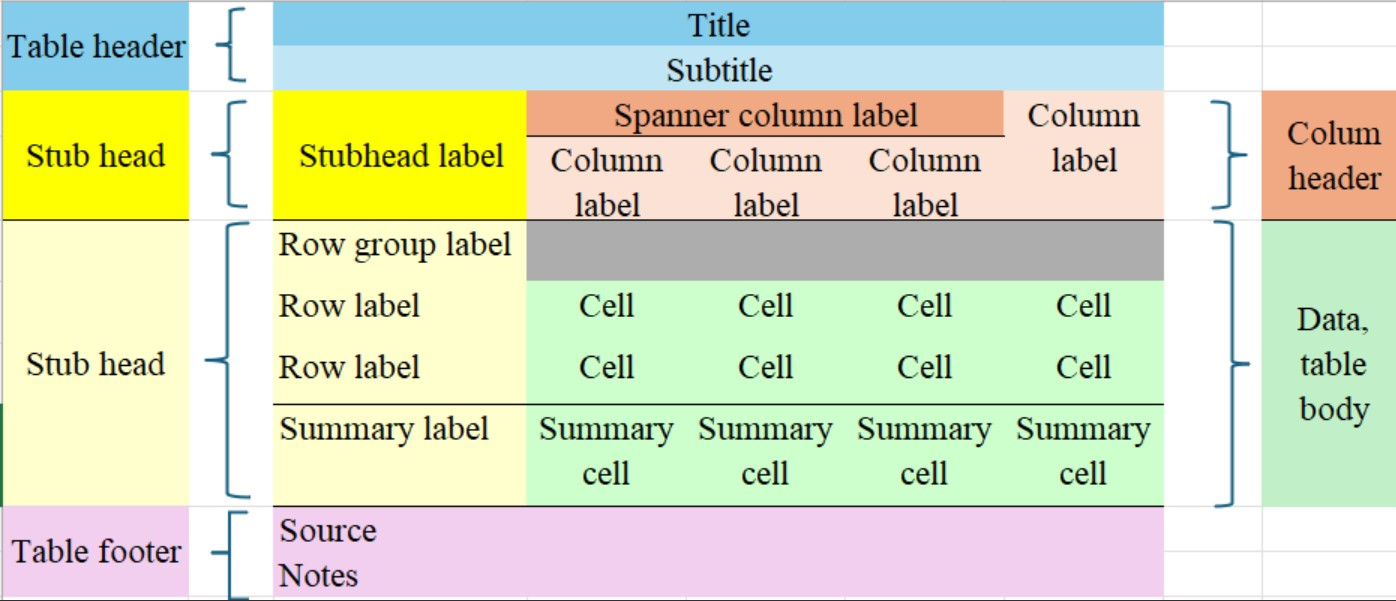
\includegraphics[width=0.5\textwidth,height=\textheight]{pics/Table1.jpg}

The following are the essential components of a well-designed table:

\begin{itemize}
\item
  The \emph{title} (and optional subtitle) of a table is mandatory and must provide a clear and precise indication of the data that will be presented in the table. These elements, combined, must answer the questions about what, where and when regarding the data to be presented inside the table. Be concise and avoid using verbs.
\item
  \emph{Column header} elements should identify the data that is displayed in each column of the table. They must also provide much of the relevant metadata: unit of measurement, time period, geographical area, etc.
\item
  \emph{Row headers} and \emph{stub} elements, provided as the first column in the table, should identify the data that is displayed in each row of the table.
\item
  \emph{Source} of the data must always be provided at the bottom of the table, and must indicate the organization responsible and the name of the survey or study that produced the results contained in the table. The omission of the citation of the source prevents the reader from seeking more information about the data presented, and should be avoided.
\item
  \emph{Notes} are optional, but they can be used to provide additional details about the data as needed to understand and use it correctly. Avoid using long texts, which if needed, would be better placed in a document that is then cited in the Notes section. If there is more than one Note, number sequentially, and use the numbers to indicate the corresponding calls inside the table. Make sure that the calls to \emph{Notes} are sufficiently distinct from the actual figures / numbers inside te table to avoid confusion.
\item
  \emph{Data} is the most important piece of information that the user expects to get from the table. Therefore, it is essential to present them in a way that is easy to extract the relevant information. For some tables, depending on the message you want to convey, it may be easier to search for information by rows or columns. This should be the most important consideration when deciding whether to present the table in portrait or landscape orientation. Dividing lines, dotted lines, shading, and even spacing can be helpful in guiding the reader to read the table in the `right' direction.
\end{itemize}

When designing tables to present statistical data, ensuring clarity and consistency is crucial. Start by maintaining uniform spacing across columns to enhance readability, while avoiding unnecessary text or excessive width that can distract from the data. Time series data should always be organized in chronological order, preferably ascending for reference tables, to provide a clear and logical progression of information. Categorize data using standard classifications to facilitate understanding and comparison across different datasets.

The arrangement of rows and columns should follow a clear and logical order, with numerical data aligned to the right to ensure decimal points are neatly aligned. Decimal places should be limited to what is necessary for precision, and rounding should aim for 3-4 significant digits to simplify the data while preserving its integrity. Avoid blank cells, which can cause confusion; instead, use appropriate symbols to indicate missing or ``not applicable'' values, ensuring the table remains informative and complete.

Finally, these practices collectively improve the usability of the table, making it easier for readers to analyze and interpret the data. By adhering to these guidelines, you create a presentation that is both professional and accessible, promoting effective communication of statistical insights.

The recommendations provided here to reference tables should also apply to longer tables provided as databases, but these can have additional resources if they are embedded on websites. For example, there may be support for users to sort tables using the values in each column, which would be useful for large tables where the user may be looking for the higher (or lower) values in a given column.

\hypertarget{dissemination-of-estimates}{%
\section{Dissemination of Estimates}\label{dissemination-of-estimates}}

National Statistical Offices routinely produce descriptive statistics, such as totals, averages, proportions, and ratios, based on survey data. These statistics provide valuable insights into key characteristics of the population, such as income levels, employment rates, or access to education. To ensure this information reaches a wide audience, NSOs often use a variety of dissemination channels, including:

\begin{itemize}
\item
  \textbf{Public Reports}: Comprehensive reports summarizing key findings from household surveys;
\item
  \textbf{Online Platforms}: Interactive data visualization tools and downloadable datasets on official websites;
\item
  \textbf{Press Releases}: Brief summaries of major findings designed to capture public and media attention.
\end{itemize}

These dissemination efforts aim to make the data understandable and actionable for policymakers, researchers, and the general public. When publishing tables of results, NSOs strive for clarity and usability. Tables are typically organized to highlight trends, comparisons, and distributions of key variables. Common features of published tables include:

\begin{itemize}
\item
  \textbf{Aggregated Data}: Grouping data by domain defining variables like age, sex, region, or socioeconomic status;
\item
  \textbf{Confidence Intervals}: Including measures of uncertainty to provide context for the estimates;
\item
  \textbf{Metadata}: Offering detailed explanations of the data collection methods, definitions, and limitations.
\end{itemize}

By presenting data in a user-friendly format, NSOs ensure their publications are accessible to a diverse audience. Chapter 10 provides more detailed discussion on presentation of survey findings. However, we note that not all estimates derived from survey data meet the necessary quality standards for publication. Estimates may be suppressed if they are based on small sample sizes, have high variance, or are otherwise unreliable. NSOs use established criteria to determine when suppression is necessary, ensuring that the released data maintains its credibility. To address this issue we can use the following approaches:

\begin{enumerate}
\def\labelenumi{\arabic{enumi}.}
\item
  \textbf{Quality Thresholds}: NSOs set predefined thresholds for measures like the coefficient of variation (CV) or standard errors;
\item
  \textbf{Flagging and Suppression}: Estimates that fall below these thresholds are either flagged with warnings about their reliability or omitted entirely from published tables;
\item
  \textbf{Transparency}: NSOs provide clear documentation explaining why certain estimates are suppressed, maintaining transparency and trust.
\end{enumerate}

\hypertarget{data-visualization}{%
\chapter{Data visualization}\label{data-visualization}}

In this section we discuss how to present data and estimates resulting from household surveys using graphics. Effective graphs can reveal patterns, trends, and relationships in the data, making it easier to interpret findings and communicate them to diverse audiences. While standard plots can still be used to show distributions and associations from the raw (unweighted) sample data, these can be misleading for the corresponding population distributions and associations. Therefore it is recommended that modified plots that account for survey weights be used instead.

For example, a bar chart showing income distribution should incorporate weights to properly represent the income distribution for the entire population. Similarly, scatter plots exploring associations between variables should use weighted markers or density adjustments to ensure the relationships are accurately depicted. In addition, regarding the display of survey estimates, which are subject to sampling error, it is important to convey this message by presenting not only point estimates, but also standard errors or confidence intervals.

When presenting survey estimates, it is essential to recognize that these estimates are subject to sampling error. To effectively communicate this uncertainty, graphs should include measures such as standard errors or confidence intervals. For instance:

\begin{itemize}
\item
  Confidence intervals can be added to bar charts or line graphs to show the range of plausible values for an estimate;
\item
  Error bars in scatter plots can illustrate the variability associated with specific data points.
\end{itemize}

Incorporating these elements into visualizations helps ensure that viewers understand the inherent uncertainty in the survey estimates, fostering more informed interpretations. When the survey units have different sampling weights, these should be taken into account when preparing graphs with their data. The main reason is that weights can be interpreted as the number of population units that each sample unit represents. Hence, it is evident that unequal weights need to be considered in the elaboration of graphs based on such sample data.

When graphs are created \emph{without} considering weights, the visual representation reflects the sample characteristics rather than the population. This discrepancy can distort distributions, proportions, or relationships between variables. Incorporating weights ensures that the graphs provide a more accurate representation of the population.

\hypertarget{bar-charts}{%
\section{Bar charts}\label{bar-charts}}

When the data of interest are categorical, their descriptive analysis will be done using contingency tables. Bar charts are commonly used to visualize categorical data. For survey data, descriptive analysis of categorical variables typically begins with contingency tables that summarize weighted counts or proportions. These tables can then be used to create bar charts, ensuring the results reflect population-level characteristics rather than just sample data. Ideally one should also aim to display error lines overlaying bars to indicate their respective confidence interval widths, thus conveying the uncertainty of the corresponding point estimates. Obtaining the weighted counts or proportions and their confidence intervals can be easily done using tools from several software packages, e.g.~the \texttt{survey} package in R.

As an example, the bar chart in Figure 9.2 presents a comparison of the number of individuals (\texttt{Nd}) between rural and urban zones, with error lines indicating the confidence intervals for each estimate. According to the values in the table, the urban zone shows a slightly higher \texttt{Nd} value than the rural zone, with 78,164 individuals in the urban area compared to 72,102 in the rural area. This difference suggests a higher concentration of people in the urban zone.

The confidence intervals allow us to assess the precision of these estimates. In the rural zone, the confidence interval ranges from 66,039 to 78,165 individuals, while in the urban zone, the confidence range goes from 72,526 to 83,802 individuals. This overlap between the intervals indicates that, although the urban zone has a higher number of individuals, the difference is not pronounced enough to be statistically significant.

Furthermore, the standard deviation of \texttt{Nd} is 3,062 for the rural zone and 2,847 for the urban zone, reflecting similar variability in both zones. This suggests that the estimates are consistent in terms of relative uncertainty, without major differences in data dispersion between the zones.

\begin{figure}
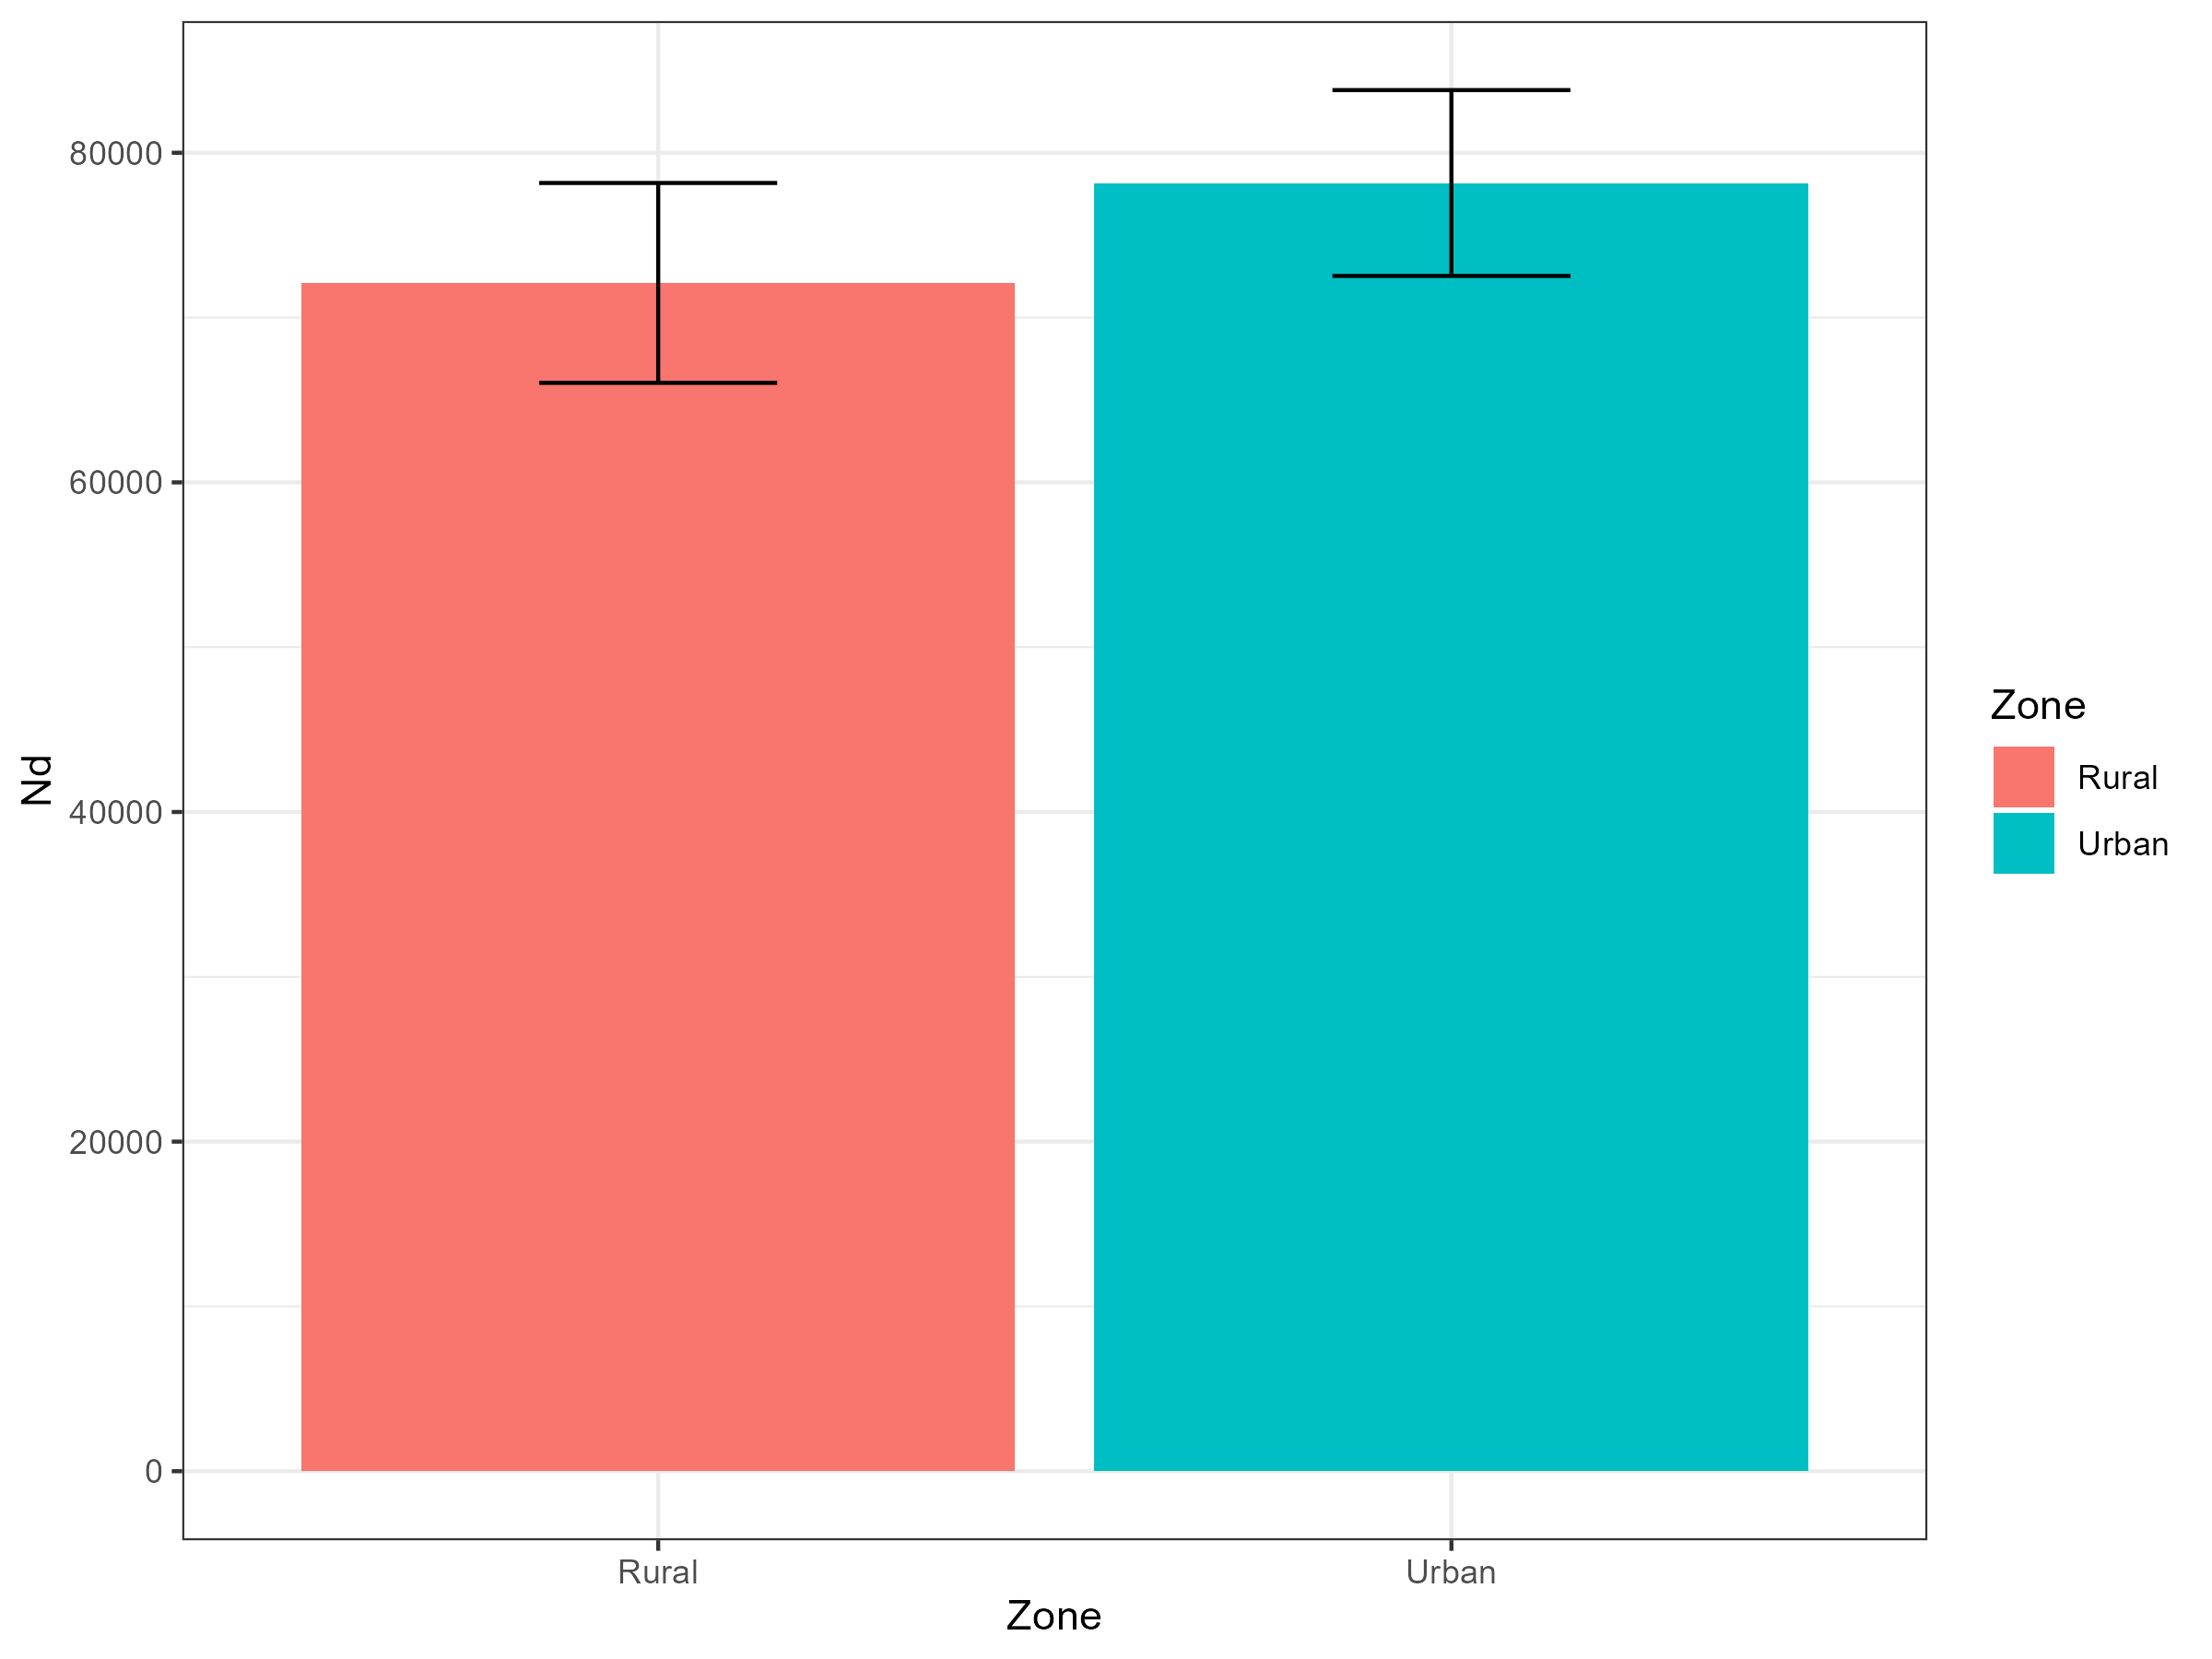
\includegraphics[width=33.33in]{www/05_graficas/03_bar_pers} \caption{Distribution of Population by Area}\label{fig:barIncome}
\end{figure}

\begin{longtable}[]{@{}
  >{\raggedright\arraybackslash}p{(\columnwidth - 8\tabcolsep) * \real{0.1944}}
  >{\raggedright\arraybackslash}p{(\columnwidth - 8\tabcolsep) * \real{0.2222}}
  >{\raggedright\arraybackslash}p{(\columnwidth - 8\tabcolsep) * \real{0.1944}}
  >{\raggedright\arraybackslash}p{(\columnwidth - 8\tabcolsep) * \real{0.1944}}
  >{\raggedright\arraybackslash}p{(\columnwidth - 8\tabcolsep) * \real{0.1944}}@{}}
\caption{Population distribution by area}\tabularnewline
\toprule\noalign{}
\begin{minipage}[b]{\linewidth}\raggedright
Zone
\end{minipage} & \begin{minipage}[b]{\linewidth}\raggedright
Number of Individuals (Nd)
\end{minipage} & \begin{minipage}[b]{\linewidth}\raggedright
Standard Error (Nd\_se)
\end{minipage} & \begin{minipage}[b]{\linewidth}\raggedright
Lower Limit (Nd\_low)
\end{minipage} & \begin{minipage}[b]{\linewidth}\raggedright
Upper Limit (Nd\_upp)
\end{minipage} \\
\midrule\noalign{}
\endfirsthead
\toprule\noalign{}
\begin{minipage}[b]{\linewidth}\raggedright
Zone
\end{minipage} & \begin{minipage}[b]{\linewidth}\raggedright
Number of Individuals (Nd)
\end{minipage} & \begin{minipage}[b]{\linewidth}\raggedright
Standard Error (Nd\_se)
\end{minipage} & \begin{minipage}[b]{\linewidth}\raggedright
Lower Limit (Nd\_low)
\end{minipage} & \begin{minipage}[b]{\linewidth}\raggedright
Upper Limit (Nd\_upp)
\end{minipage} \\
\midrule\noalign{}
\endhead
\bottomrule\noalign{}
\endlastfoot
Rural & 72,102 & 3,062 & 66,039 & 78,165 \\
Urban & 78,164 & 2,847 & 72,526 & 83,802 \\
\end{longtable}

\hypertarget{histograms}{%
\section{Histograms}\label{histograms}}

Histograms serve to present the distribution of a single numeric (continuous) survey variable or response. If one had a census, then the histogram is a powerful tool to describe the underlying distribution, even for very large datasets. When displaying sample data, however, the sampling weights must be taken into account when estimating frequencies or relative frequencies of population units having values in the specified histogram bins. Modern survey analysis tools can easily provide weighted histograms where the sampling weights are incorporated.

Histograms are often seen as precursors to density function estimates. A density estimate can be thought of as a histogram with a large number of bins, providing a smoother view of the data distribution. The \texttt{survey} package in R includes functionality for plotting smoothed density estimates that account for sampling weights, offering a more detailed representation of the population.

A common example of visualization in this type of analysis is the use of histograms to represent the distribution of variables such as income. These charts allow us to observe the distribution of the variable of interest in the expanded population and to understand its shape, dispersion, and general trends.

It is also common to perform graphical analyses broken down by subgroups, such as geographic areas (urban and rural) or thematic characteristics like sex (male and female). This approach helps identify key differences among specific population subgroups, for instance, by examining income distribution in men and women over the age of 18. Such breakdowns help visualize and communicate potential gaps between subgroups of interest.

In this way, charts help to communicate results in an accessible manner, offering a clear and straightforward visual representation for audiences who may not be familiar with the technical details of estimation methods.

In \ref{fig:histIncome} the horizontal axis (x) represents income levels, spanning from 0 to over 4000 monetary units, while the vertical axis (y) indicates frequency, meaning the number of individuals within each income range.

The distribution shows that most of the population is concentrated at lower income levels, with a particularly high frequency near 0. As income levels rise, frequency declines sharply, indicating a right-skewed (positively skewed) distribution with a smaller proportion of people at higher income levels. The light gray bars visually emphasize this concentration at lower incomes, highlighting a significant disparity in the population's income distribution.

\begin{figure}
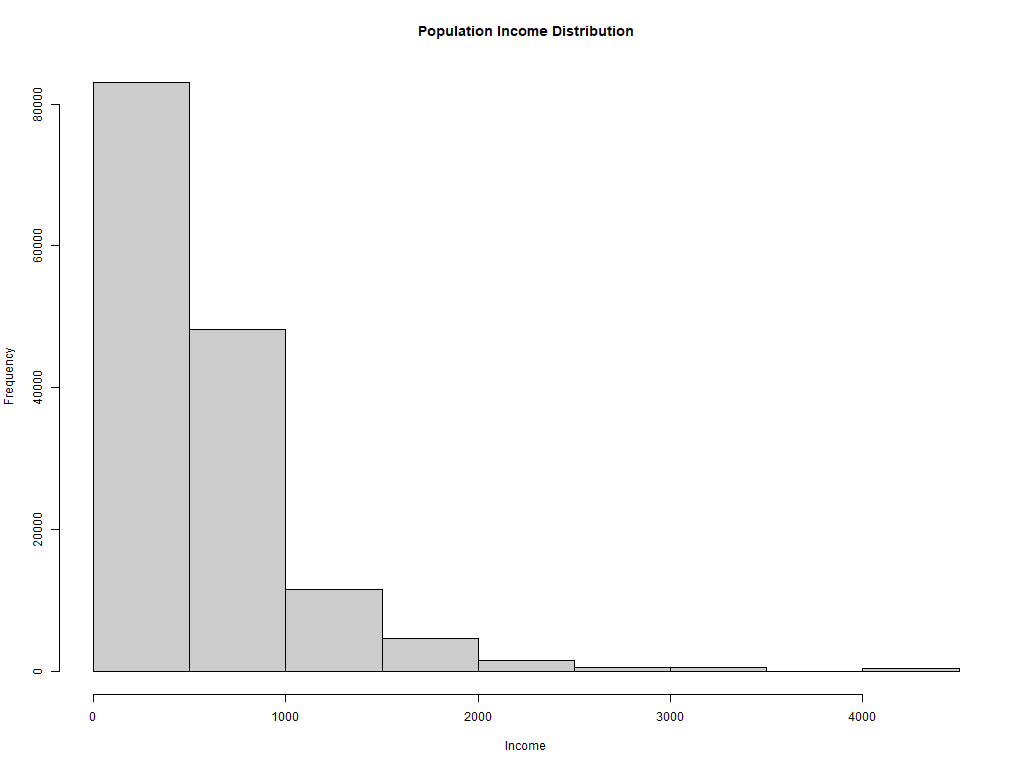
\includegraphics[width=14.22in]{www/05_graficas/01_hist_ingreso} \caption{Distribution of Population Income}\label{fig:histIncome}
\end{figure}

As an example, Figure \ref{fig:HistIncomeExpenditureSex} presents two histograms illustrating the distribution of income and expenditure by sex. In the histogram on the left, titled ``Income Histograms by Sex,'' we observe the income distribution, where blue bars represent men and pink bars represent women. The majority of the population, both male and female, is concentrated in the lower income levels, showing a right-skewed distribution. In the lower income levels, there are more men than women, while at higher income levels, the difference is less pronounced.

In the histogram on the right, titled ``Expenditure Histograms by Sex,'' the distribution of expenditure is shown, also broken down by sex. Similar to income, most of the population of both sexes is concentrated in the lower expenditure levels, with a right-skewed trend. There is also a higher proportion of men in the lower expenditure levels, while at higher levels, the representation between sexes is more balanced. These histograms exemplify the similarity in the income and expenditure distributions between men and women, although men appear to be slightly more represented in the lower levels of both variables.

\begin{figure}
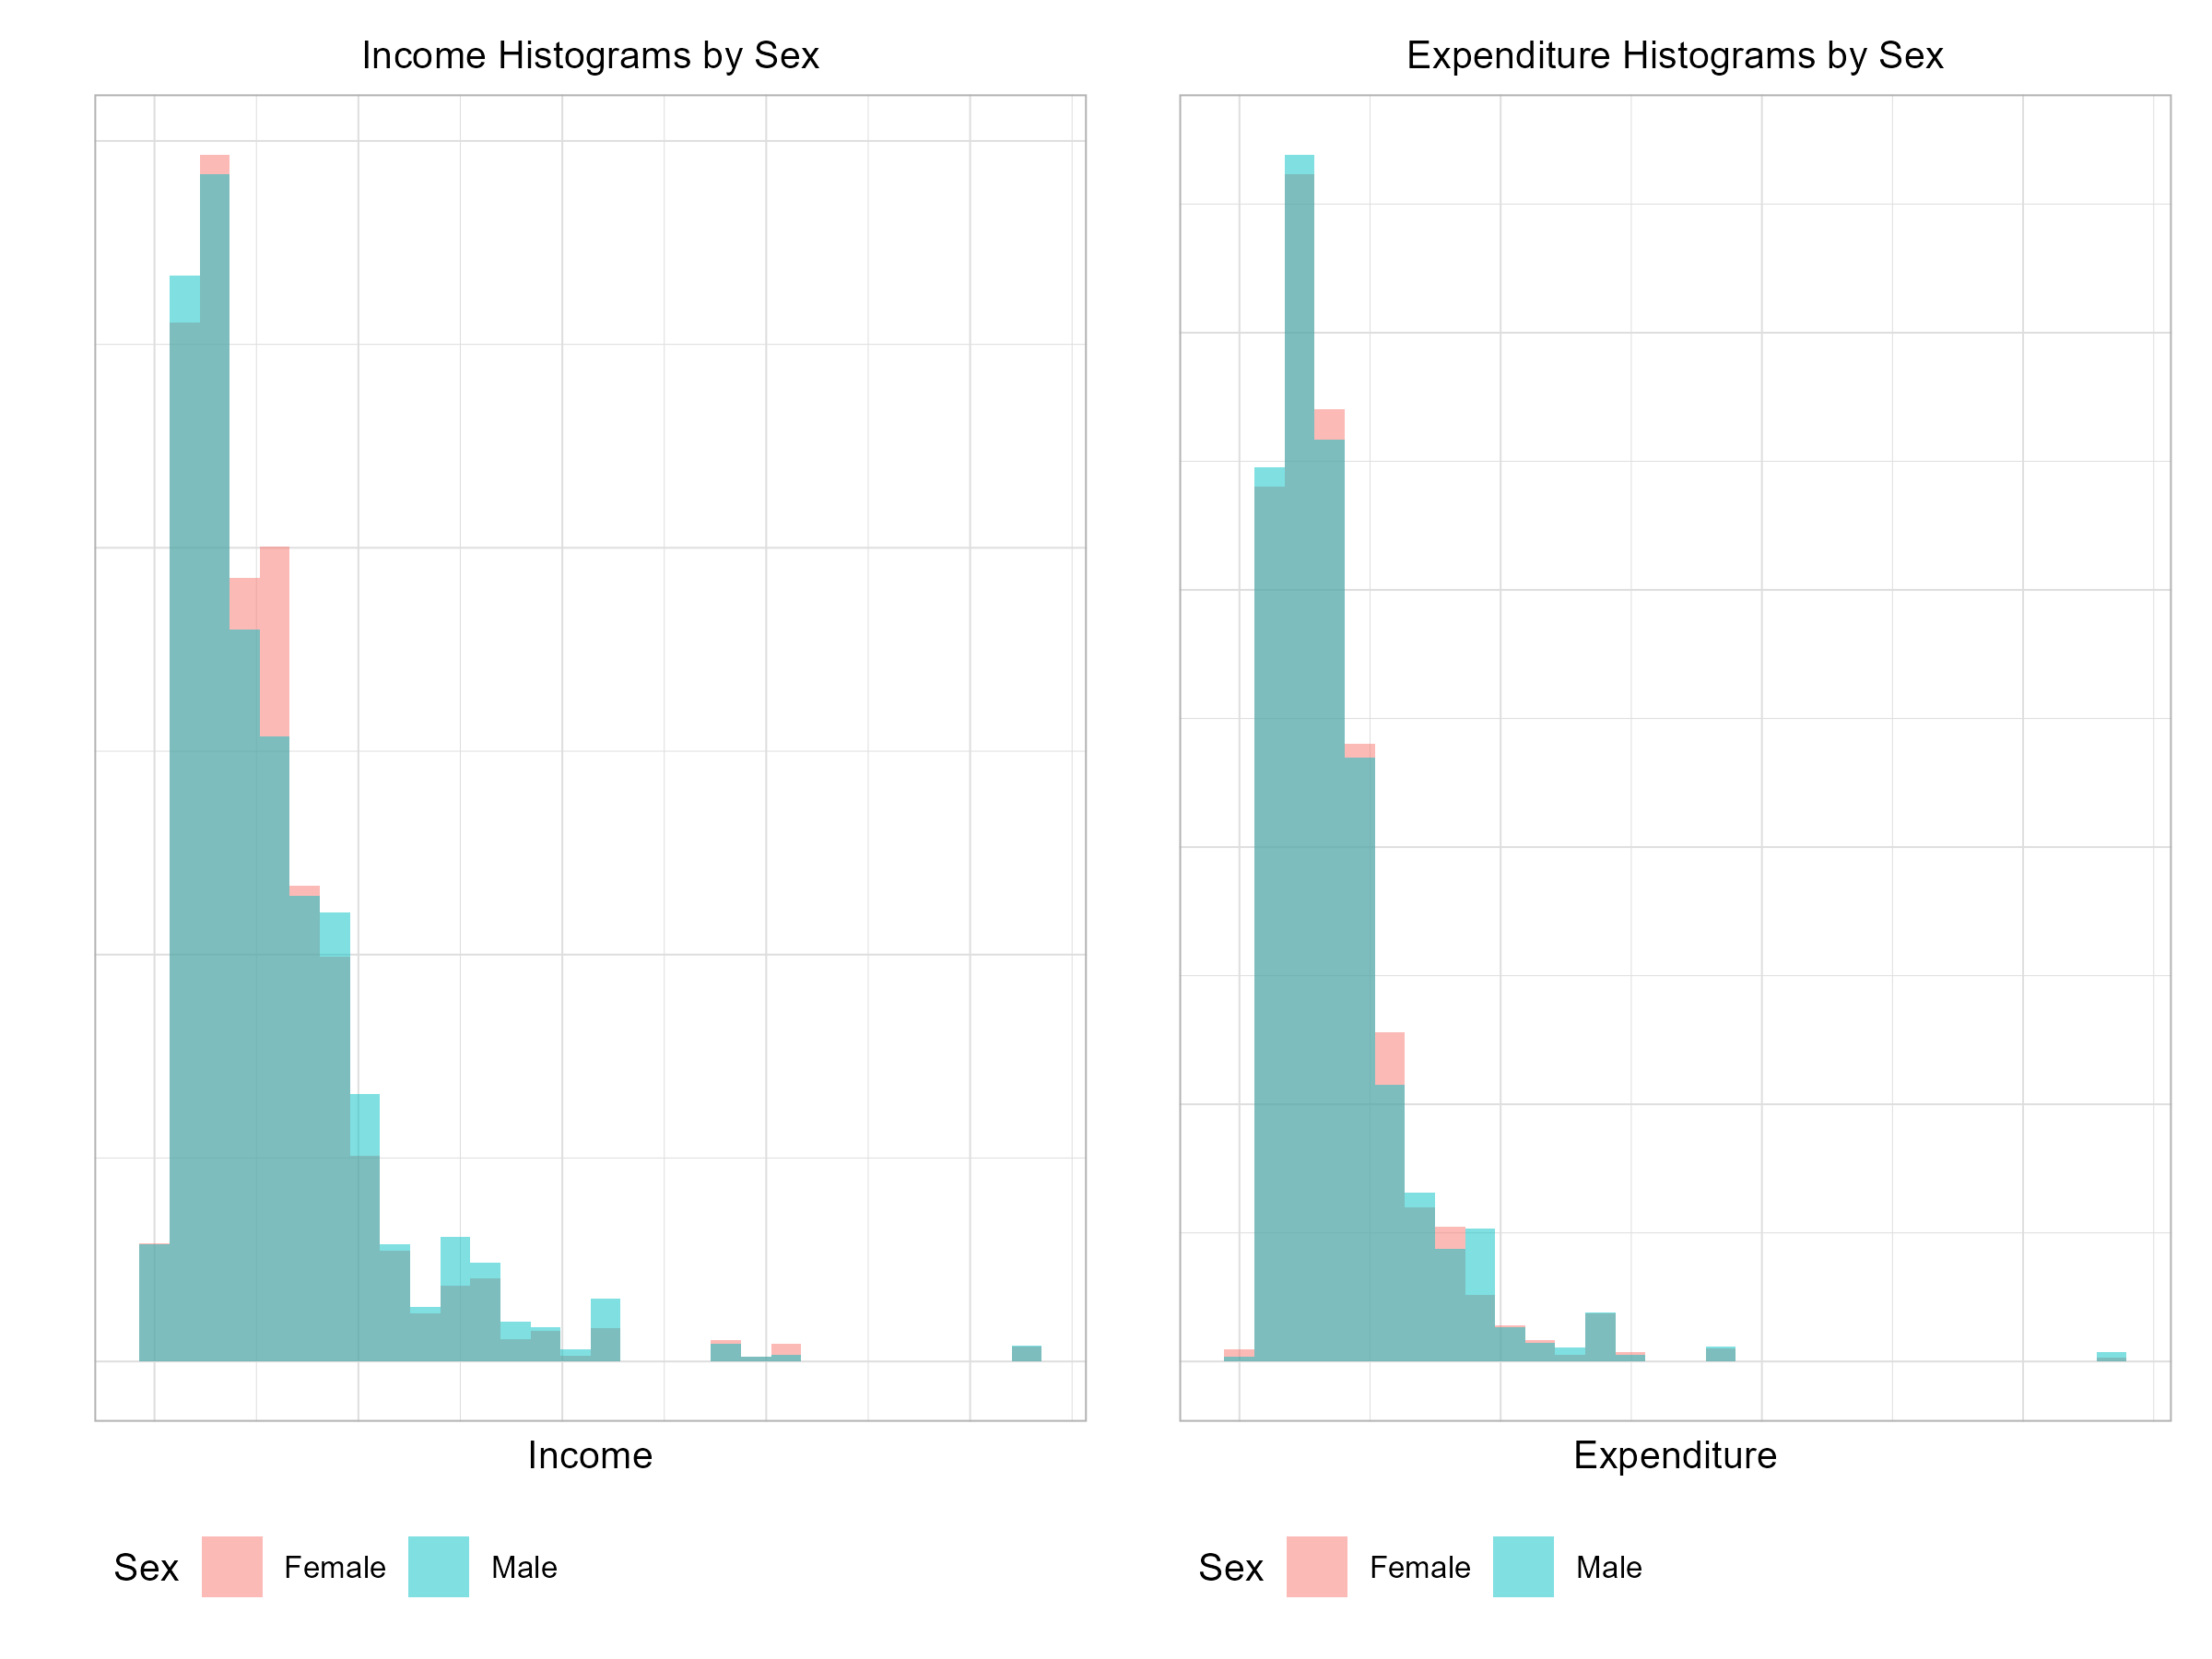
\includegraphics[width=33.33in]{www/05_graficas/02_Hist_sex} \caption{Histograms of Income and Expenditure by Sex}\label{fig:HistIncomeExpenditureSex}
\end{figure}

Histograms, especially when weighted for survey design, are invaluable for exploring and presenting the distribution of continuous variables. Subgroup analyses further enhance their utility, enabling the identification of disparities and trends across different population segments. Combined with smoothed density estimates, histograms provide a comprehensive and accurate view of the population's numeric variables.

\hypertarget{scatter-plots}{%
\section{Scatter Plots}\label{scatter-plots}}

Scatter plots are the tool of choice to explore relationships between two continuous variables, potentially revealing patterns or trends in the data. These plots face the two challenges discussed above. First one needs to try and convey in the plot that the different sample observations carry different weights. For small to moderate sample sizes this can be done by plotting circles or dots of varying sizes where the symbol size represents the corresponding observation sampling weight. Plots like these can be obtained using standard bubble plot tools or the scatter plot available in the \texttt{survey} package in R. As stated by \citet{Lumley2010}, when dealing with large datasets, displaying all the data points in a scatter plot can be overwhelming and cluttered. Several strategies can help address this issue:

\begin{enumerate}
\def\labelenumi{\arabic{enumi}.}
\item
  \textbf{Subsampling}: Select a smaller, manageable subsample from the full dataset. The subsample should be selected with probabilities proportional to the sampling weights, ensuring that it behaves approximately like a simple random sample from the population. The resulting scatter plot maintains representativeness while being easier to interpret. The subsample obtained in this way behaves approximately as a simple random sample from the survey population.
\item
  \textbf{Hexagonal Binned Scatter Plots}: Divide the plot area into a grid of hexagons. Instead of plotting individual points, represent each hexagon with shading or size based on the total sampling weights of the points within that hexagon. This approach condenses the data into a clear and interpretable visualization. With complex household survey data, the number of points in a hexagonal bin should be replaced by the sum of the weights for points in the bin.
\item
  \textbf{Smoothed Scatter Plots}: Avoid plotting individual points altogether and instead estimate and display trends. For example, calculate specific quantiles (e.g., quartiles) of the y-axis variable conditioned on the x-axis variable and smooth these values across the range of the x-axis. This approach highlights trends while minimizing visual clutter.
\end{enumerate}

The figure \ref{fig:ScatterIncome}, illustrates the weighted relationship between income and expenditure in a population. In this plot, the size of the points represents the weight assigned to each observation. A high concentration of points is observed at lower income and expenditure levels, suggesting that most of the population has low income and low expenditure.

Although there is an upward trend, indicating that income and expenditure tend to increase together, the dispersion of points reveals that higher expenditure is not always associated with proportionally higher income. Some larger points, corresponding to observations with greater weight, are distributed across different levels of income and expenditure without concentrating in a single area. Additionally, a few isolated points at high expenditure levels may represent outliers with considerably higher-than-average expenditure. Overall, this plot suggests a positive relationship between income and expenditure, accompanied by significant variability and some exceptional cases.

\begin{figure}
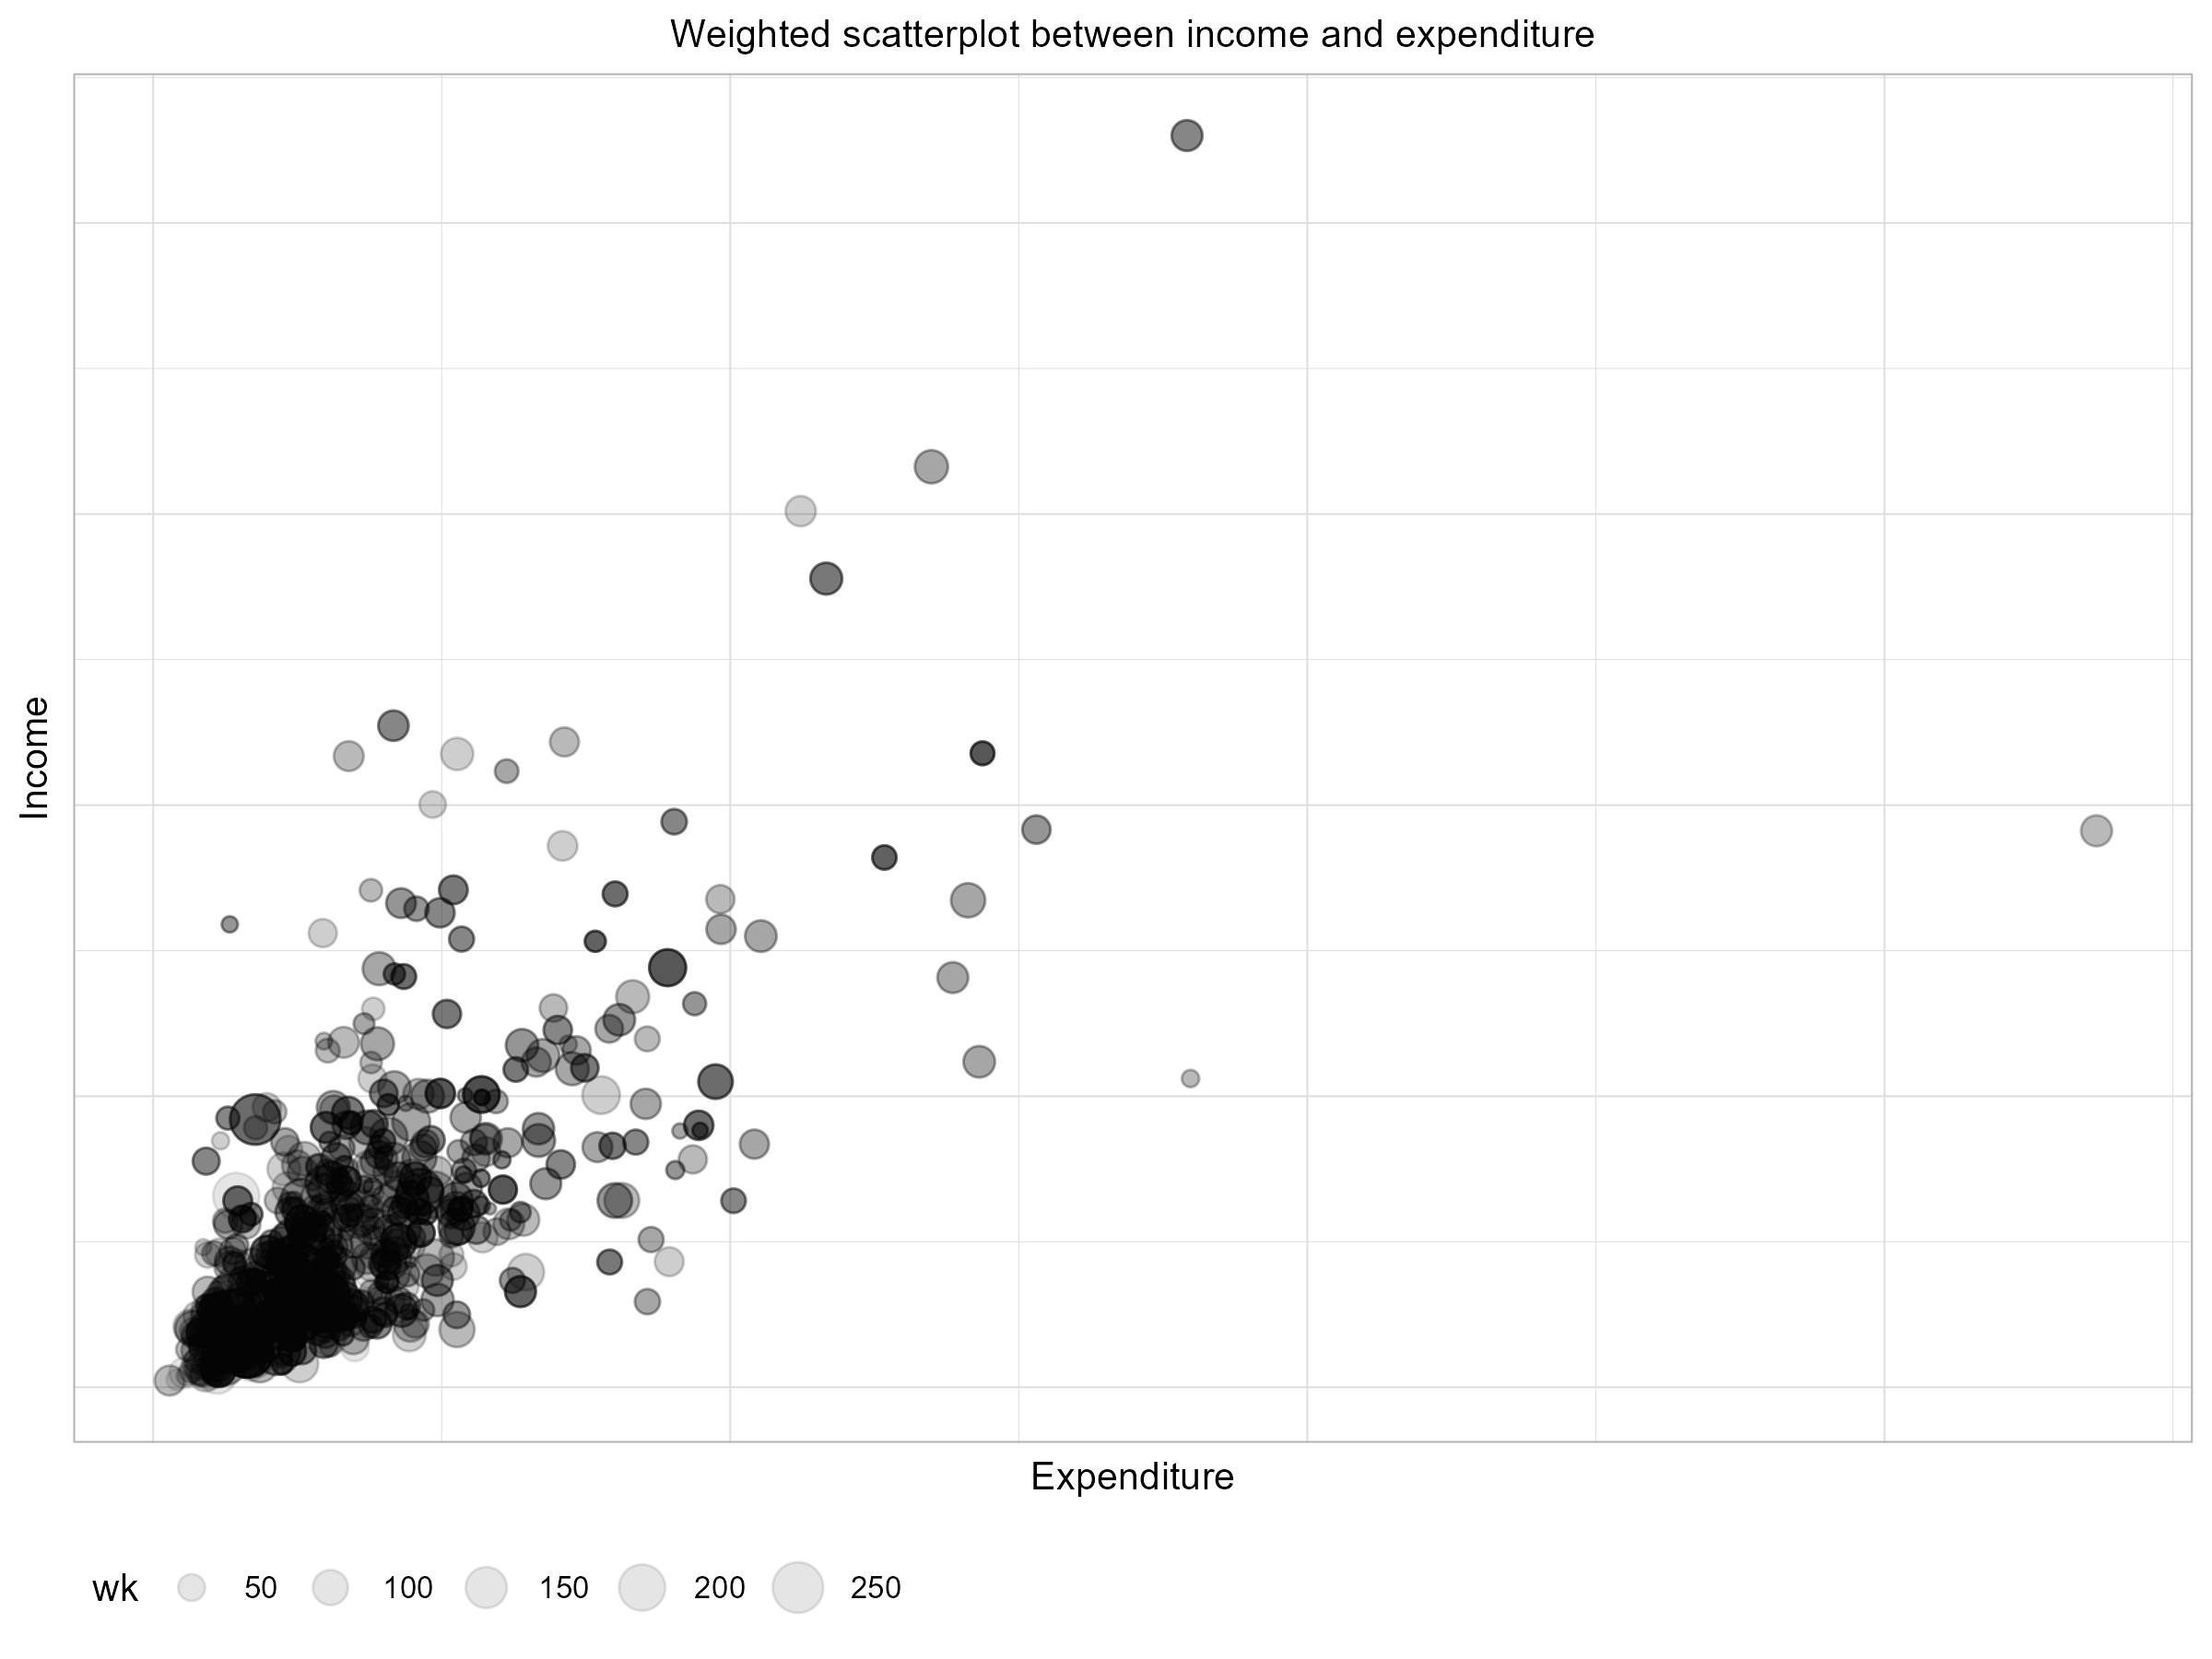
\includegraphics[width=33.33in]{www/05_graficas/02_scatterplot_ingreso_gasto} \caption{Weighted scatterplot between income and expenditure}\label{fig:ScatterIncome}
\end{figure}

Scatter plots are a versatile and effective way to explore relationships between variables in survey data. By incorporating sampling weights and adopting strategies to manage large datasets, they can provide clear, meaningful insights into population-level patterns. Whether using weighted points, hexagonal binning, or smoothing techniques, scatter plots remain a cornerstone of data visualization for continuous variables.

\hypertarget{nso-practical-example-2}{%
\section{NSO -- Practical example}\label{nso-practical-example-2}}

In this subsection we will include the experience of a NSO on displaying information through graphics.

\hypertarget{references}{%
\chapter*{References}\label{references}}
\addcontentsline{toc}{chapter}{References}

  \bibliography{chapterbib.bib}

\end{document}
